\documentclass[10pt]{report}
\usepackage[utf8]{inputenc}
\usepackage[spanish]{babel}
\usepackage[top=1.2cm,bottom=1.2cm,left=1.2cm, right=1.2cm]{geometry}
\usepackage{nopageno}

\usepackage{amsmath,amssymb}

% Imágenes
\usepackage{graphicx}
% Justificar texto
\usepackage{ragged2e}
% BibLaTex
\usepackage{biblatex,csquotes}
\addbibresource{Referencias.bib}

\usepackage{listings}
\usepackage{color}
\usepackage{lscape}

\definecolor{dkgreen}{rgb}{0,0.6,0}
\definecolor{gray}{rgb}{0.5,0.5,0.5}
\definecolor{mauve}{rgb}{0.58,0,0.82}

\lstset{frame=tb,
	language=Python,
	aboveskip=3mm,
	belowskip=3mm,
	showstringspaces=false,
	columns=flexible,
	basicstyle={\small\ttfamily},
	numbers=none,
	numberstyle=\tiny\color{gray},
	keywordstyle=\color{blue},
	commentstyle=\color{dkgreen},
	stringstyle=\color{mauve},
	breaklines=true,
	breakatwhitespace=true,
	tabsize=3
}

\begin{document}
	
\begin{center}
	\vspace*{1cm}
	
	{\fontsize{12}{14} \textbf{CIC-IPN}}
	
	\vspace{0.2cm}
	
	{\fontsize{12}{14} \textbf{Tarea número 2}}
	
	\vspace{0.2cm}
	
	{\fontsize{14}{16} \textbf{Reconocimiento de Formas y Visión por Computadora}}
	
	\vspace{0.1cm}
	
	Alumno: Valle Martínez Luis Eduardo
	
	\vspace{0.1cm}
	
	Profesor titular: Dr. Humberto Sossa
	
	\vspace{0.1cm}
	
	Fecha de entrega: 17 de Junio del 2022
	
\end{center}

\hfill \break

\section*{Introducción}
	\subsection*{Tecnologías utilizadas}
	\hfill\break
	\justifying
	El presente documento funciona como reporte de la tarea número 2 asignada en el curso de RFVC.
	
	\hfill\break
	\justifying
	Retomando la infraestructura creada para los objetivos de la primer práctica, se desarrollan los nuevos requisitos del programa añadiendo funcionalidad al programa básico de tratamiento de imágenes.
	
	\hfill\break
	\justifying 
	Se recuerda del primer programa codificado su desarrollo en los lenguajes: Python y QML. Python fue utilizado eclusivamente para los procesos de tratamiento de imágenes, ya sea desarrollando métodos propios o explotando las herramientas disponibles en la biblioteca especializada \textbf{OpenCV}. Así también este lenguaje sirve para la coordinación entre los procesos lógicos y los eventos de la interfaz visual.
	
	\hfill\break
	\justifying
	QML por su parte, como lenguaje de diseño de aplicaciones enfocado en la interfaz de usuario y con un paradigma declarativo, se integra en el \textit{framework} \textbf{PySide6} con soporte para la compatilidad con Python, y que su principal responsabilidad es la de manejar eventos de usuario, actualizaciones de interfaz y demás situaciones relacionadas con la GUI. Utilizando lo que se denomina \textit{Slots}, se logra la ejecución de procesos en el \textit{backend}, y este comunicando a su vez sus resultados con \textit{Signals} hacia la GUI.
	
	\hfill\break
	\justifying
	Del proyecto previo se destacan las funcionalidades disponibles(todas manejables desde un componente en la GUI) que permiten la integración de los nuevos requisitos de esta segunda entrega:
	\begin{itemize}
		\item Apertura imágenes en la GUI para su manejo
		\item Visualizado de los datos de la imagen(Nombre, tamaño en px, formato)
		\item Elección de los colores del pixel en la imagen
		\item Conversión a escala de grises de una imagen
		\item Binarización de la imagén con un umbral especificado
		\item Contabilización de objetos
		\item Recuperado del histograma de la imagen
	\end{itemize}
	
	\subsubsection*{Requisitos para ejecución}
		\begin{itemize}
			\item Python version 3.9.7
			\item Biblioteca \textbf{Numpy}
			\item Biblioteca \textbf{Matplotlib}
			\item Biblioteca \textbf{OpenCV}(4.5.5)
			\item Biblioteca \textbf{PySide6} para la GUI
		\end{itemize}
	
		Una vez instaladas las bibliotecas, dentro de la carpeta de código se puede ejecutar el comando en una terminal:
		
		\begin{verbatim}
 $ python3 main.py
		\end{verbatim}

\subsection*{Objetivo de la práctica}
	\hfill\break
	\justifying
	Implementar funciones básicas del tratamiento de imágenes pertenecientes a etapas de Preprocesamiento y Segmentación, según el paradigma de Gonzalez y Woods.
	
	\hfill\break
	\justifying
	No obligatorio pero si práctico en función de la infraestructura que provee la práctica previa, se integran las nuevas funcionalidades en el programa con interfaz gráfica, facilitando en buena medida su comprensión y uso.
	
	\hfill\break
	\justifying
	Guiándose por los requisitos planteados para esta práctica, se añaden procesos de 6 tareas principalmente, siendo descrito su comportamiento y la solución alcanzada al exponerse a fondo cada una de ellas en su sección particular en páginas siguientes.
	
\subsection*{Interfaz gráfica}
	\hfill\break
	\justifying
	Sin cambios en paleta de colores o estilo de la interfaz, se implementan nuevas secciones colapsables dividiendo las diferentes tareas y sus funciones que se ponen a disposición del usuario.
	\begin{figure}[htbp]
		\centering
		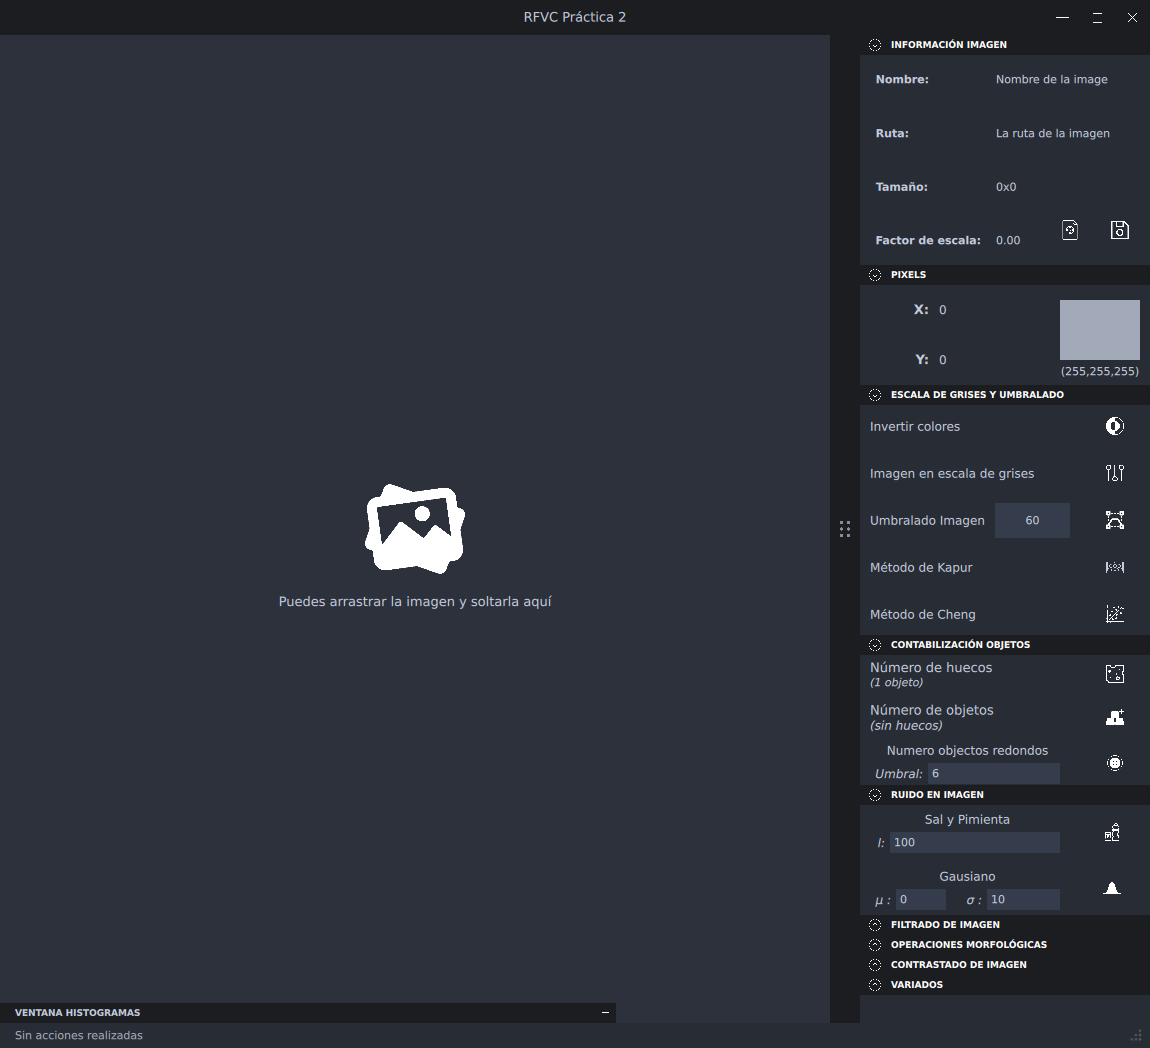
\includegraphics[width=18cm]{Imagenes/GUI.png}
		\caption{Ventana gráfica de la GUI al ejecutarse el programa.}
	\end{figure}
	

\newpage

\section*{1. Escala de grises y umbralado}
	\hfill\break
\justifying
Integrando el escalado en grises, inversión de los colores y los métodos manuales y automáticos de umbralado, se tratan a fondo los métodos de umbralado automático únicamente, y aunque la funcionalida de inversión de colores es una función reciente, su implementación es tan sencilla como la negación por bit de su valor en la imagen. Otro enfoque más sencillo consiste en restar a 255 el valor actual de cada pixel.

\subsection*{Método de Kapur}
	\hfill\break
	\justifying
	Esta técnica de umbralado se utiliza cuando en una imagen se encuentran 2 tendencias de los niveles en escalas de grises, una perteneciente al fondo y la otra al objeto, para esto los objetos deben tener un buen contraste respecto al fondo.
	
	\hfill\break
	\justifying
	La umbralización automática de Kapur, se centra en encontrar un valor para el umbral \textit{u}, tal que la división dicotómica de clases para una imagen basándose en los valores de grises de los píxeles según su histograma, seá la maximización de la medida de la información utilizando le ecuación de la entropía como medida de la información.
	
	\hfill\break
	\justifying
	Se define a la entropía de la imagen completa como:
	\begin{equation*}
		H_T = -\sum_{r=0}^{L-1} p_r ln(p_r)
	\end{equation*}
	
	\hfill\break
	\justifying
	La información de las 2 clases es: $I(C_1,C_2)=H_{C_1}(u)+H_{C_2}(u)$. La definición de la entropía de cada clase son las ecuaciones:
	{\large \begin{equation*}
		\begin{array}{r l l}
			H_{C_1}(u)= & -\overset{u}{\underset{r=0}{\sum}}\frac{p_r}{p(C1)}ln\left( \frac{p_r}{p(C1)} \right) & = lnp(C_1)+\frac{H_u}{p(C1)}\\
			H_{C_2}(u)= & -\overset{L-1}{\underset{r=u+1}{\sum}}\frac{p_r}{1-p(C1)}ln\left( \frac{p_r}{1-p(C1)} \right) & = lnp(1-C_1)+\frac{H_t-H_u}{1-p(C1)}\\
		\end{array}
	\end{equation*}}
	Con $C_1$ como la probabilidad acumulada de los valores de los pixeles hasta el índice \textit{u}.

	\hfill\break
	\justifying
	Ambas ecuaciones como la suma de la información de cada clase se puede rescibir como un funcional:
	{\Large \begin{equation*}
		J_k(u) = ln[p(C_1)(1-p(C_1))]+\frac{H(u)}{p(C_1)}+\frac{H_T-H(u)}{1-p(C_1)}
	\end{equation*}}
	
	\hfill\break
	\justifying
	Buscando el valor de \textit{u} donde el funcional es máximo:
	{\Large \begin{equation*}
		u* = arg \underset{0 \leq u \leq L-1}{max} J_k(r)
	\end{equation*}}

	\hfill\break
	\justifying
	Su implementación se logra de manera sencilla utilizando las operaciones y propiedades que proveén los arreglos de la biblioteca numpy. Con funciones completamente vectorizadas, se determina el valor del umbral \textit{u} en muy poco tiempo y además con un código muy descriptivo parecido a las propias ecuaciones.
	
	\begin{lstlisting}[language=Python]
	def kapur_threshold(image):
		# Probability of each pixel value
		p,_ = histogram(image, bins=range(256), density=True)
		# Cumulative probabilities for C1 and C2
		c1 = p.cumsum(); c2 = 1.0 - c1
		# When the probabilities are 0 its changed to 1 so that it won't affect when used as divider
		c1[c1 <= 0] = 1; c2[c2 <= 0] = 1
		# Entropy of the image
		#   To avoid the case: ln(0)
		#   And as the entropy for each pixel values is p*ln(p)
		#   the values of p that are 0 are changed to 1 so when the entropy its
		#   applied the this pixel value won't affect the whole entropy
		#   ** The entropy of the whole image will be the last element of H_u
		p_1 = copy(p); p_1[p_1 == 0.0] = 1
		H_u = -(p_1*log(p_1)).cumsum()
		H_t = H_u[-1]
		# Functional
		#   Jk(u) = H_c1(u)+H_c2(u) = ln(c1*c2)+[H(u)/c1]+[(H_t-H(u))/c2]
		Jk = log(c1*c2)+(H_u/c1)+((H_t-H_u)/c2)
		return argmax(Jk)
	\end{lstlisting}

	\hfill\break
	\justifying
	Las pruebas del método de Kapur, otorgaron resultados mas bien malos para la umbralización de una imagen en clases dicotómicas, con valores de \textit{u} muy altos o muy bajos, para la imagen que se maneja. Se utilizan como ejemplos para este método 3 ímagenes sencillas obtenidas del banco de imágenes del propio Dr. Humberto Sossa, que describen objetos completamente negros de diferentes geometrías sobre un fondo color claro y unos palillos de paleta.
	
	\begin{figure}[!h]
		\begin{tabular}{cc}
			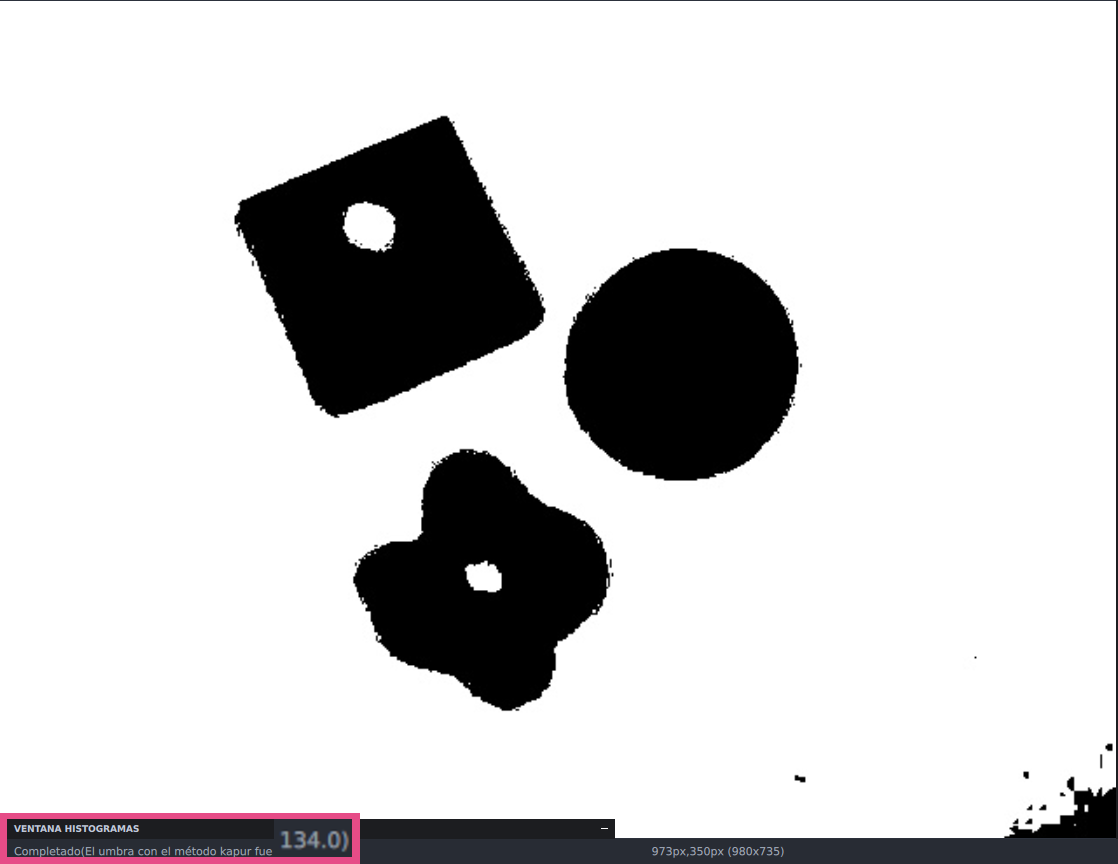
\includegraphics[width=9.5cm]{Imagenes/Kapur_1.png} & 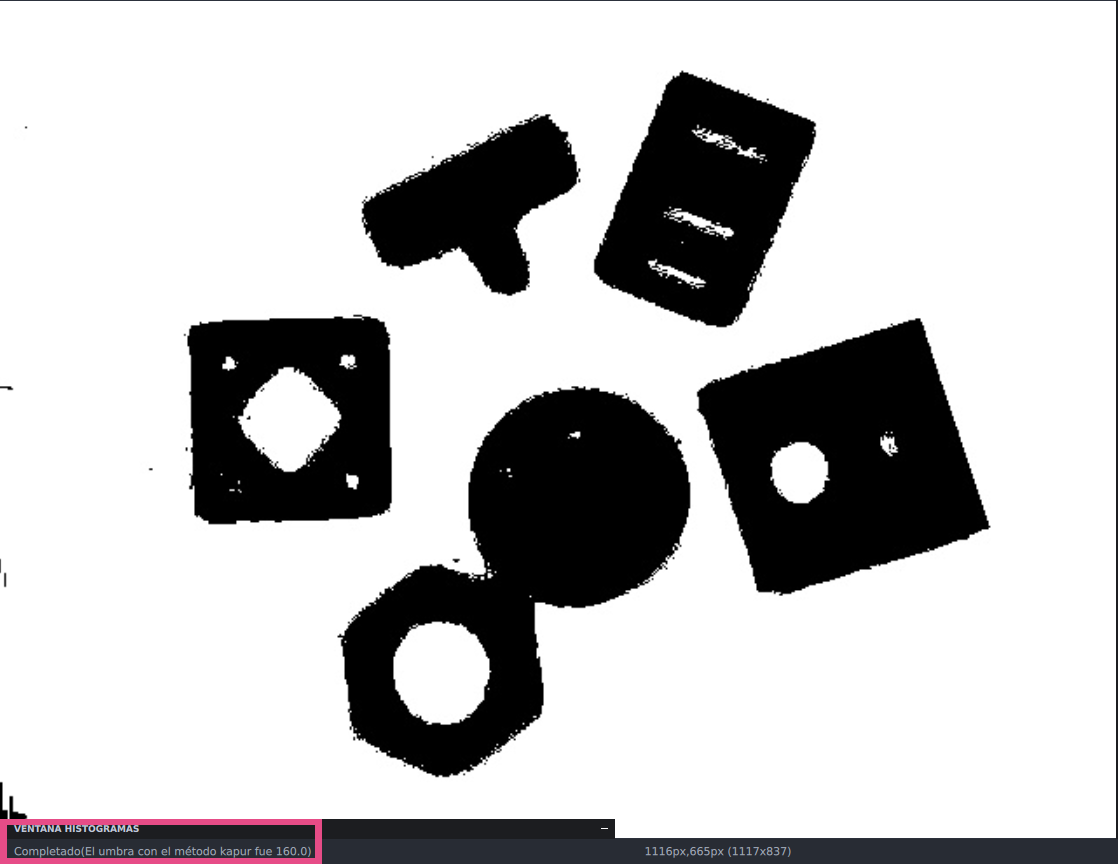
\includegraphics[width=9.5cm]{Imagenes/Kapur_2.png} \\
			\multicolumn{2}{c}{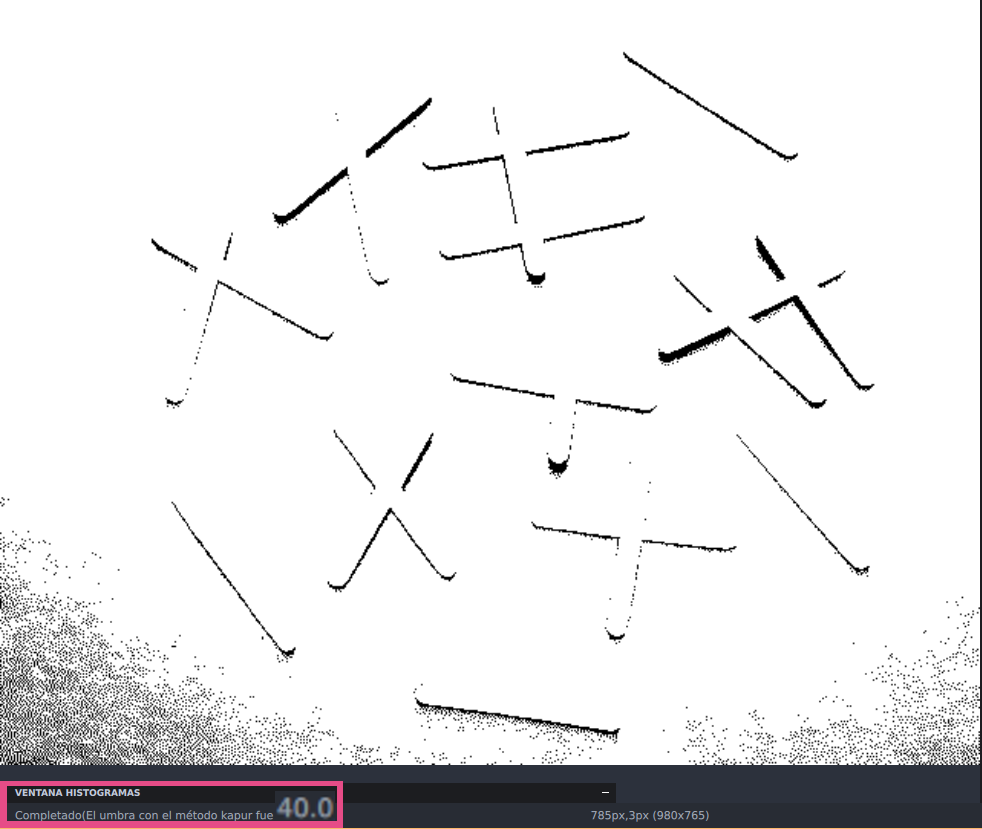
\includegraphics[width=10cm]{Imagenes/Kapur_3.png}}
		\end{tabular}
		\label{Kapur}
		\caption{Resultados obtenidos de la aplicación del método de Kapur para la umbralización automática. \\ 1) 3 objetos negros constrastados con un fondo claro. Se obtuvo un umbral muy grande(134) \\ 2) 6 objetos negros constrastados con un fondo claro. Se obtuvo un umbral muy grande(160) \\ 3) Palos de paleta claros con un fondo obscuro. Se obtuvo un umbral muy pequeño(40)}
	\end{figure}
	
\subsection*{Método de Cheng}
	\hfill\break
	\justifying
	Al igual que sucede con el método de Kapur, el método de Cheng se utiliza en el umbralado dicotómico, aunque es expandible a un entorno multiclase. En este trabajo se implementa de solo 2 modas.
	
	\hfill\break
	\justifying
	En esta técnica de binarización automática, los pixeles se suponen variables aleatorias de las que se puede calcular la correlación y a través de las distribuciones de probabilidad $C_1$ y $C_2$ se describe la cantidad de esta.
	
	\hfill\break
	\justifying
	Se recuerda que la correlación se puede calcular como:
	\begin{equation*}
		C(X) = -ln\sum_{r\geq1} p_r^2
	\end{equation*}
	Por lo tanto para cada distribución se define:
	\begin{equation*}
		\begin{aligned}
			G(u) = \sum_{r=1}^{u} p_r^2 \\
			G'(u) = \sum_{r=u+1}^{L-1} p_r^2 \\
		\end{aligned}
	\end{equation*}
	
	\hfill\break
	\justifying
	Como se intenta obtener la máxima correlación entre el objeto de interés y el fondo se realiza la suma de correlaciones para cada clase:
	\begin{equation*}
		CT(u) = C_{C_1}(u) + C_{C_2}(u)
	\end{equation*}
	Pudiendose calcular de la siguiente forma entonces:
	{\Large \begin{equation*}
		\begin{aligned}
			CT(u) = -ln\sum_{r=1}^{u} \left( \frac{p_r}{P_1(u)} \right)^2 -ln\sum_{r=u+1}^{L-1} \left( \frac{p_r}{1-P_1(u)} \right)^2 \\ = -ln[G(u)\times G'(u)]+2ln[P1(u)\times(1-P_1(u))]
		\end{aligned}
	\end{equation*}}
	
	\hfill\break
	\justifying
	Finalmente el umbral se obtiene de identificar el argumento del funcional que maximiza la correlación:
	{\Large \begin{equation*}
		u* = arg \underset{0\leq u \leq L-1}{max} CT(r)
	\end{equation*}}
	
	\hfill\break
	\justifying
	Muy similar a como sucede con Kapur, este método facilmente puede implementarse utilizanando operaciones y propiedades de los array de la biblioteca numpy, facilitando la operación, expresión y optimizando en operaciones pues estas son sumamente veloces.
	
	\begin{lstlisting}[language=Python]
	def cheng_threshold(image):
		# Frecuency of each pixel value
		_,p = histogram_no_image(image)
		# The filter for reducing 0 gets applied
		p = mean_filter(p)
		# Probabilities of each pixel value
		p = p/p.sum()
		# Cumulative probabilities for C1 and C2
		c1 = p.cumsum(); c2 = 1.0 - c1
		# Cumulative sum of the square of pixels probability and the complement
		G = (p**2).cumsum(); G_c = G[-1]-G
		# When the probabilities are 0 its changed to 1 so that it
		# won't affect when used inside the natural logarithm
		c1[c1 <= 0] = 1; c2[c2 <= 0] = 1
		G[G == 0] = 1; G_c[G_c == 0] = 1
		# Functional
		# CT(u) = C_c1(u)+C_c2(u) = -ln[G(u)xG'(u)]+2ln[P1(u)+P2(u)]
		CT = -log(G*G_c) + 2*log(c1*c2)
		return argmax(CT)
	\end{lstlisting}
	
	\hfill\break
	\justifying
	Las pruebas del método de Chen, al igual que el de Kapur, otorga resultados deficientes con valores de \textit{u} muy altos o muy bajos, lo que sugiere que se utilizen otro tipo de métodos como Kittler e Illinworth para la binarización automática de imagenes con 2 modas.
	
	\begin{figure}[!h]
		\begin{tabular}{cc}
			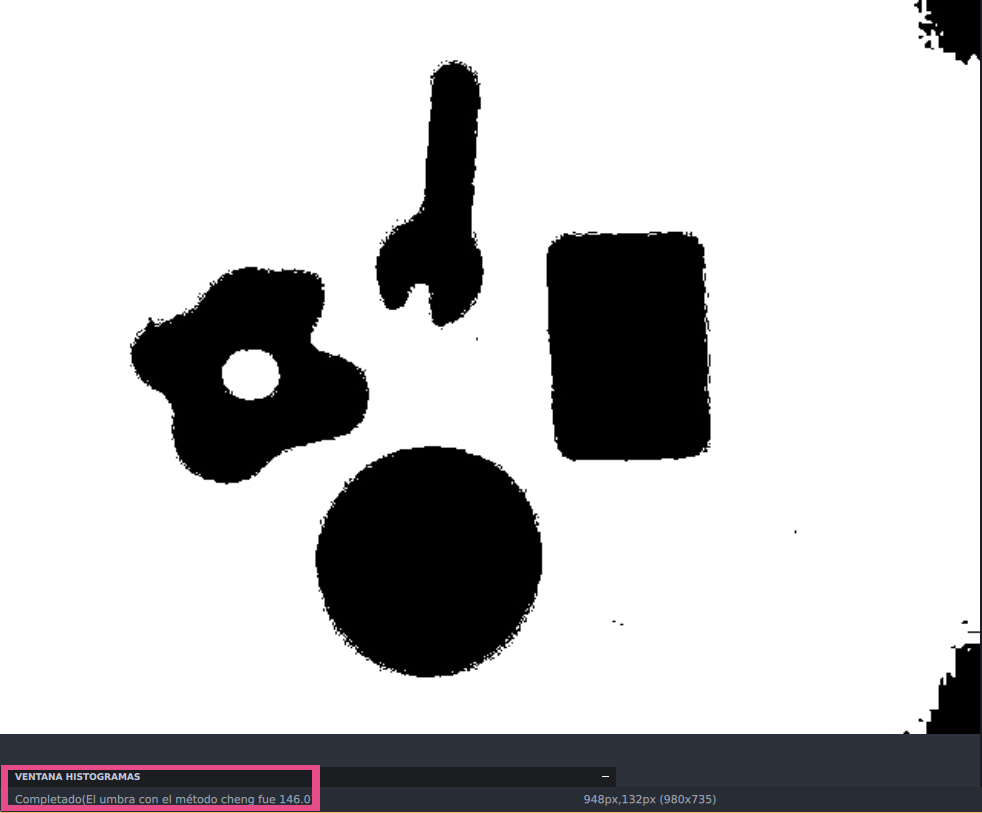
\includegraphics[width=10cm]{Imagenes/Cheng_1.png} & 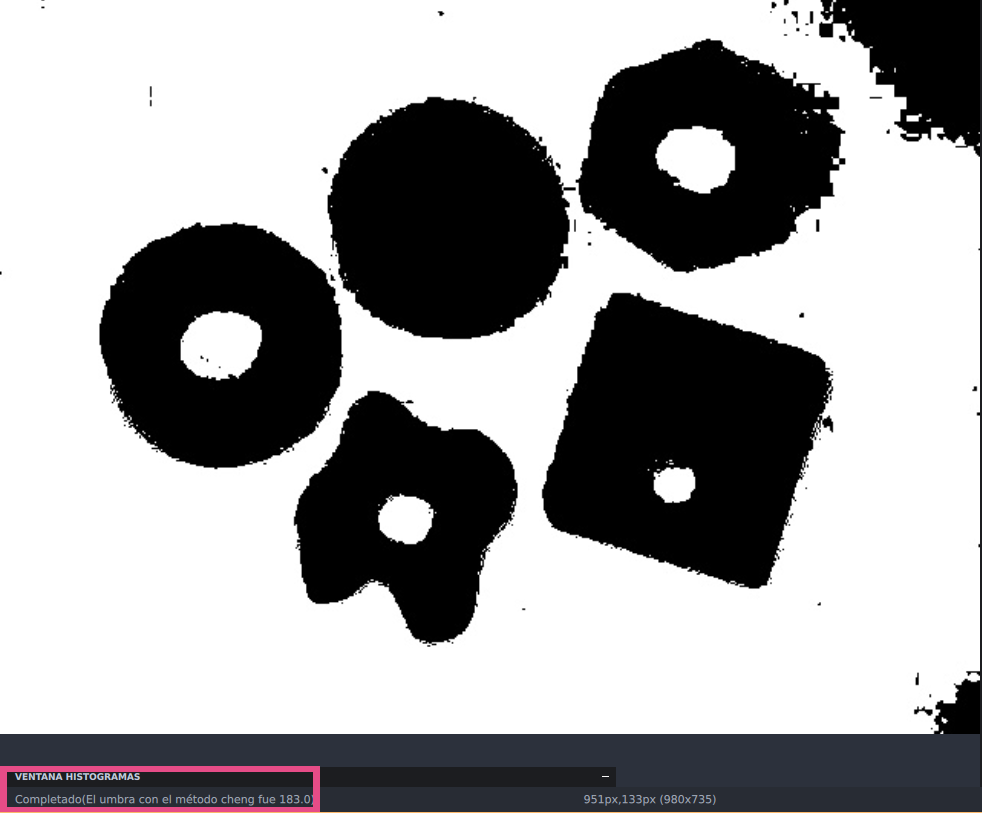
\includegraphics[width=9cm]{Imagenes/Cheng_2.png} \\
			\multicolumn{2}{c}{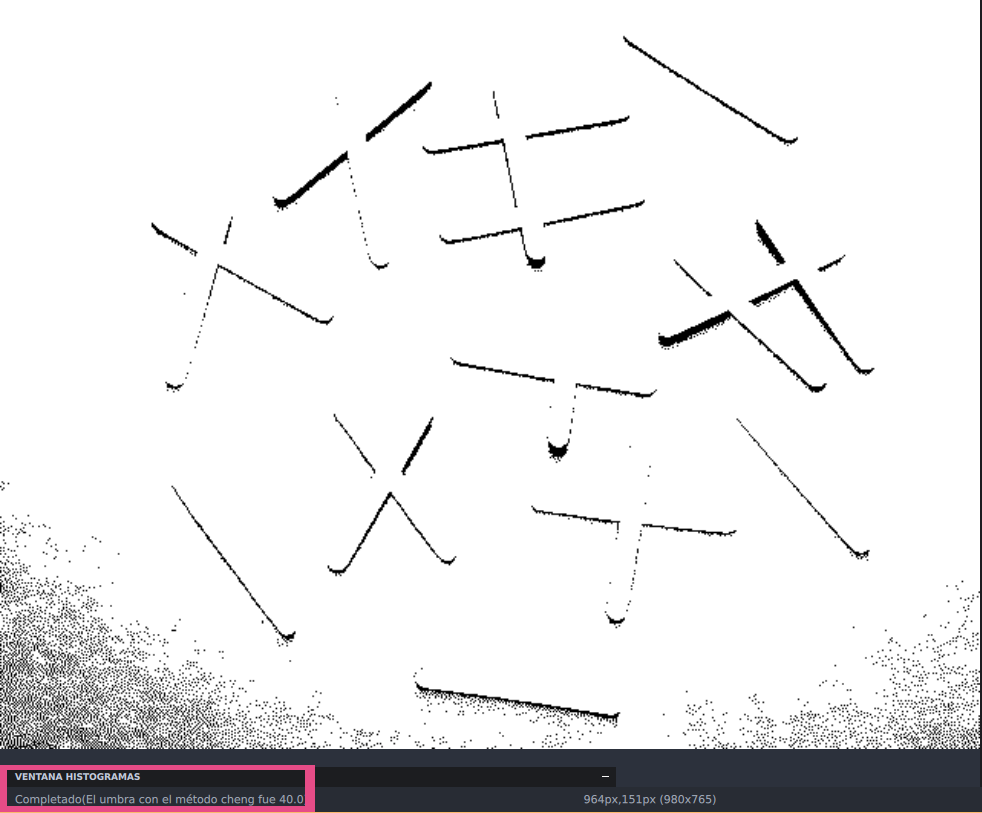
\includegraphics[width=11cm]{Imagenes/Cheng_3.png}}
		\end{tabular}
		\label{Cheng}
		\caption{Resultados obtenidos de la aplicación del método de Cheng para la umbralización automática. \\ 1) 4 objetos negros constrastados con un fondo claro. Se obtuvo un umbral muy grande(146) \\ 2) 5 objetos negros constrastados con un fondo claro. Se obtuvo un umbral muy grande(183) \\ 3) Palos de paleta claros con un fondo obscuro. Se obtuvo un umbral muy pequeño(40)}
	\end{figure}
	
\newpage
	
\section*{2. Contabilización Objetos}
	\input{Contabilizacion_objetos}
	
\newpage
	
\section*{3. Ruido en imagen}
	\hfill\break
\justifying
Siguiendo en el orden de secciones, se encuentran las operaciones capaces de adicionar ruido a las imagenes.´

\hfill\break
\justifying
Aún cuando el ruido en una imagen es un factor detrimental, es una situación muy común en la captura de imagenes por lo que su estudio es también importante y es así que se agregan la funcionalidad para adicionamiento de ruido.

\hfill\break
\justifying
El ruido, como cualquier entidad o resultado que es intermedio en una imagen capturada, no es de interes para los propósitos del cómputo principal, por lo que se suele definir al ruido como toda a quella situación que entorpece en cualquiera de las etapas, al tratamiento de las imágenes.

\hfill\break
\justifying
Con diversas causantes que pueden generar ruido en nuestras imagenes, se mencionan los tipos de ruidos clasificados en 3:
\begin{itemize}
	\item \textbf{Aditivo}: Se adiciona al azar a cada pixel de la imagen $f(x,y)$, un valor real \textit{c}, de forma que: $\overbrace{f}(x,y) = f(x,y)+c$.
	
	\textbf{Substractivo}: Se resta en este caso, al azar a cada pixel de la imagen $f(x,y)$, un valor real \textit{c}, de forma que: $\overbrace{f}(x,y) = f(x,y)-c$
	
	\textbf{Mezclado}: Se adiciona o resta al azar a cada pixel de la imagen $f(x,y)$, un valor real \textit{c}, de forma que: $\overbrace{f}(x,y) = f(x,y)+c$ o $\overbrace{f}(x,y) = f(x,y)-c$
\end{itemize}

\hfill\break
\justifying
Con la finalidad de estudiarlos y entender las técnicas que pueden ayudar a contrarrestrarlos, se añaden los ruidos más comunes:

\subsection*{Ruido Gausiano}
	\hfill\break
	\justifying
	Produce pequeñas variaciones en la image, generalmente tiene origen en los componentes electrónicos. Afecta a la imagen completa donde la desnsidad de todos los pixeles se ve alterada. Cada muestra de entrada es afectada por un valor diferente, desde cero hasta un valor de saturación mínimo o máximo.
	
	\hfill\break
	\justifying
	Este tipo de ruido mezclado, sigue un comportamiento gausiano, de forma que la variable \textit{c} toma valores según la siguiente relación:
	\begin{equation*}
		c = (L-1)exp\left( \frac{-z^2}{2\sigma^2} \right)
	\end{equation*}

\subsection*{Ruido Sal y Pimienta}
	\hfill\break
	\justifying
	El valor que toma el pixel no tiene relación con el valor real, sino que toma valores muy altos o muy bajos. Tomando el máximo(sal) o el mínimo(pimienta). Se produce normalmente en la cuantificación que se realiza en el proceso de digitalización.
	
	\hfill\break
	\justifying
	Como este tipo de ruido se caracteriza por saturar el valor de uno o más pixeles de la imagen hacia los límites positivos o límite inferior, su asignación se realiza en el programa de forma aleatoria con el valor de \textit{l} como limitante de cuanto ruido de este tipo adicionar

\subsection*{Implementacion ruido}
\hfill\break
\justifying
La implementación del proceso de adicionado de ruido para cada tipo es diferente, más sin embargo se conjuntan ambos en 1 sola función por la facilidad que ofrece este tipo de implementación. Para adicionar uno u otro, se pasa un parámetro tipo \textit{string} con la cadena \textit{'gaussian'} o \textit{'s\&p'} para escoger el tipo, mientras que los parámetros de cada uno se pasa como valor con llave, situación en la que Python deja su adición en la llamada a la función sin poner límite a estos mientras se especifique la lista en la definición de la función.

\newpage

	\begin{landscape}
		\begin{figure}[!h]
			\begin{tabular}{cc}
				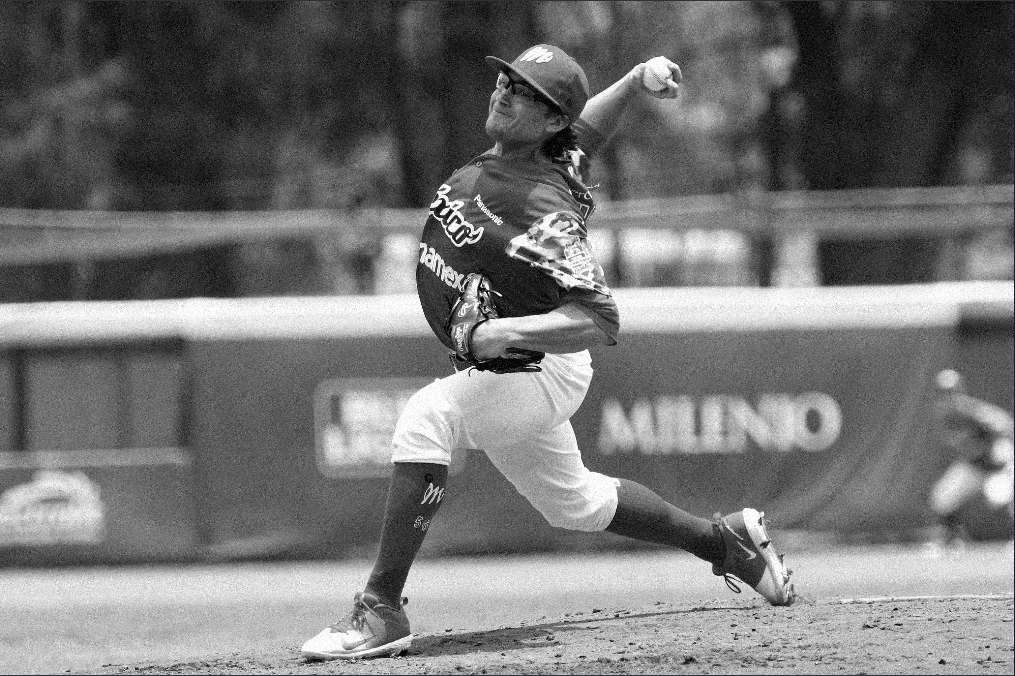
\includegraphics[width=12.25cm]{Imagenes/Ruido_gauss_bn_1.png} & 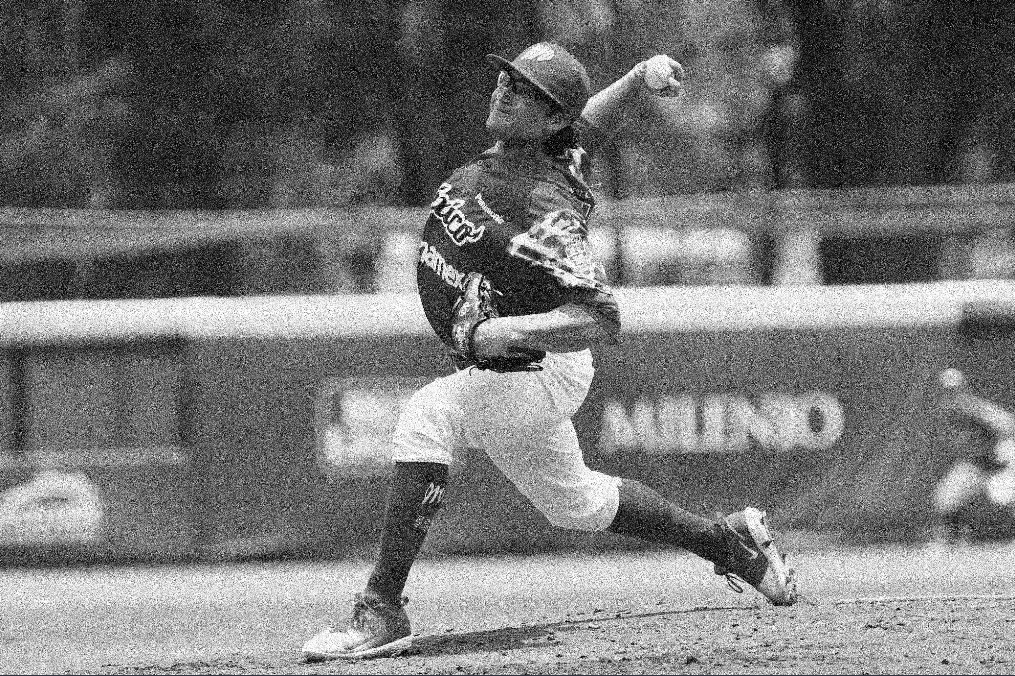
\includegraphics[width=12.25cm]{Imagenes/Ruido_gauss_bn_2.png} \\
				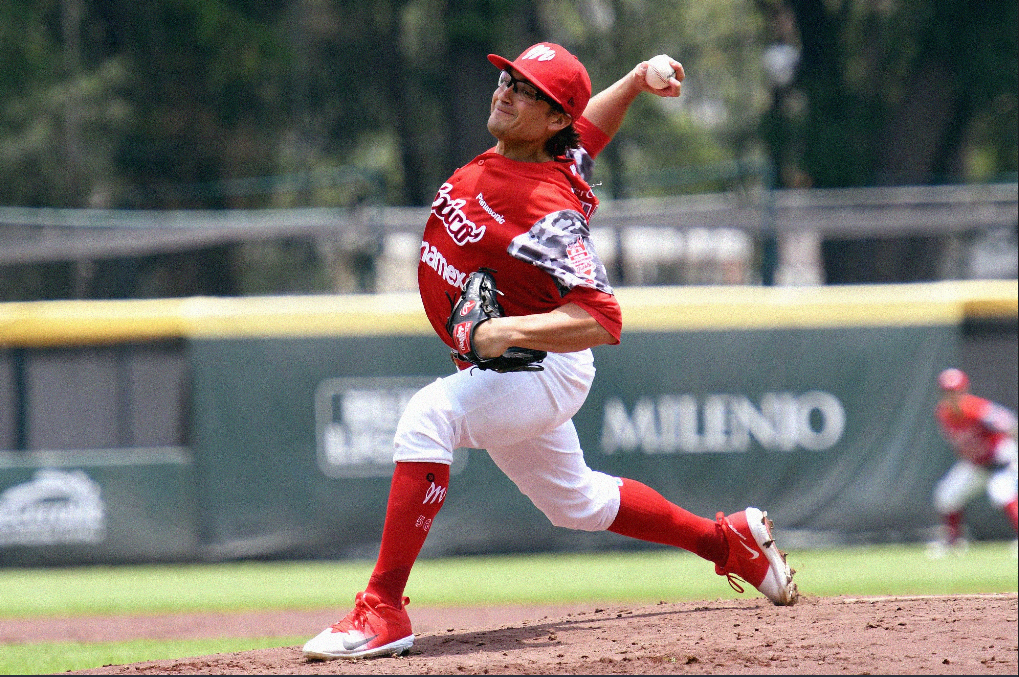
\includegraphics[width=12.25cm]{Imagenes/Ruido_gauss_color_1.png} & 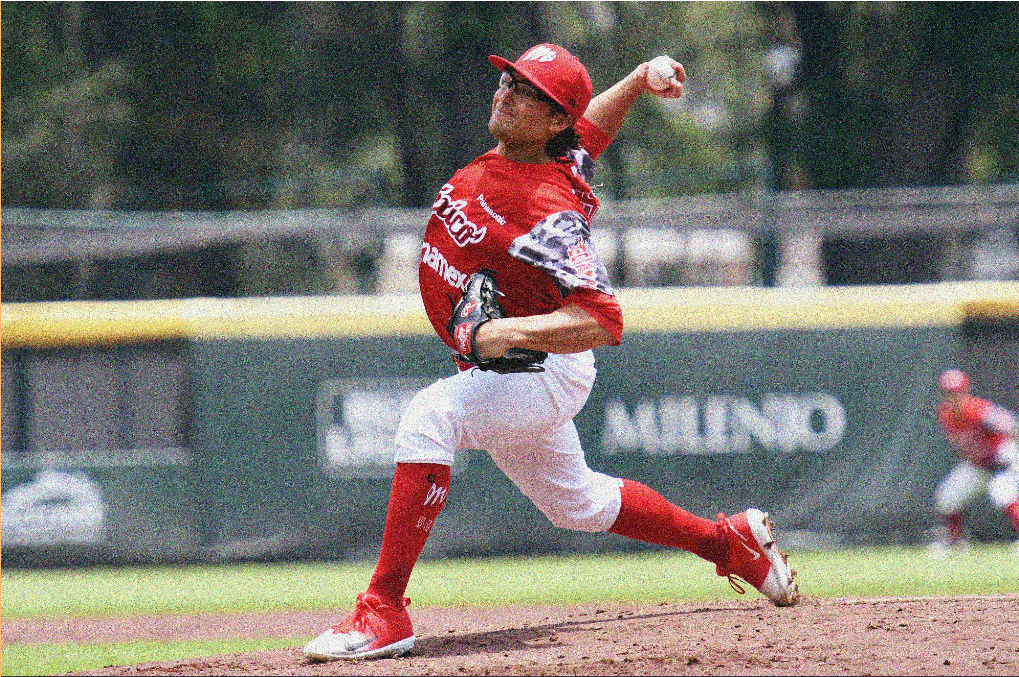
\includegraphics[width=12.25cm]{Imagenes/Ruido_gauss_color_2.png}
			\end{tabular}
			\label{Ruido_Gauss}
			\caption{Ejemplo de imágenes a escala de grises y a color, con ruido tipo gaussiano adicionado \\ 1) Imagen en escala de grises con parámetros $\mu= 3$ y $\sigma = 15$ \\ 2) Imagen en escala de grises con parámetros $\mu= 5$ y $\sigma = 50$ \\ 3) Imagen a color con parámetros $\mu = 3$ y $\sigma = 15$ \\ 4)Imagen a color con parámetros $\mu = 5$ y $\sigma = 50$}
		\end{figure}
	\end{landscape}

	\begin{landscape}
		\begin{figure}[!h]
			\begin{tabular}{cc}
				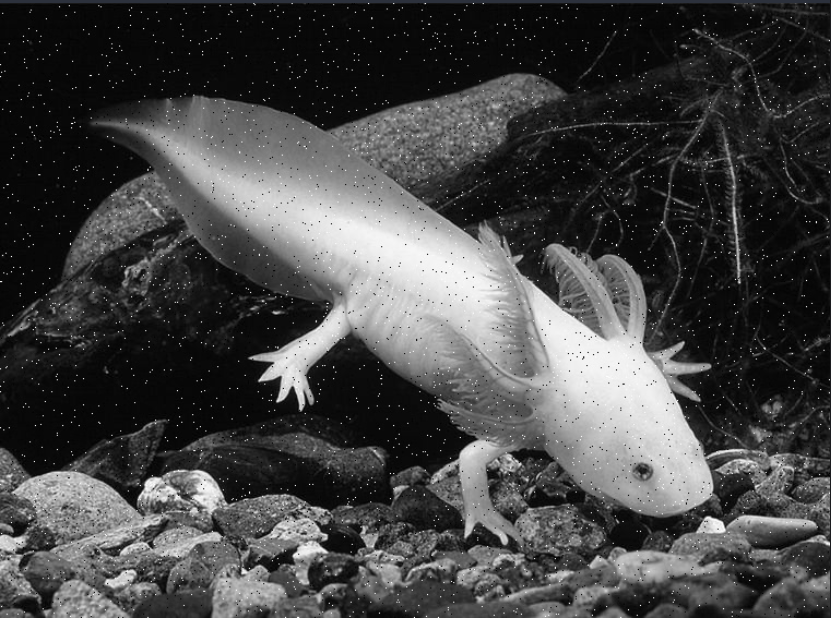
\includegraphics[width=11cm]{Imagenes/Ruido_sp_bn_1.png} & 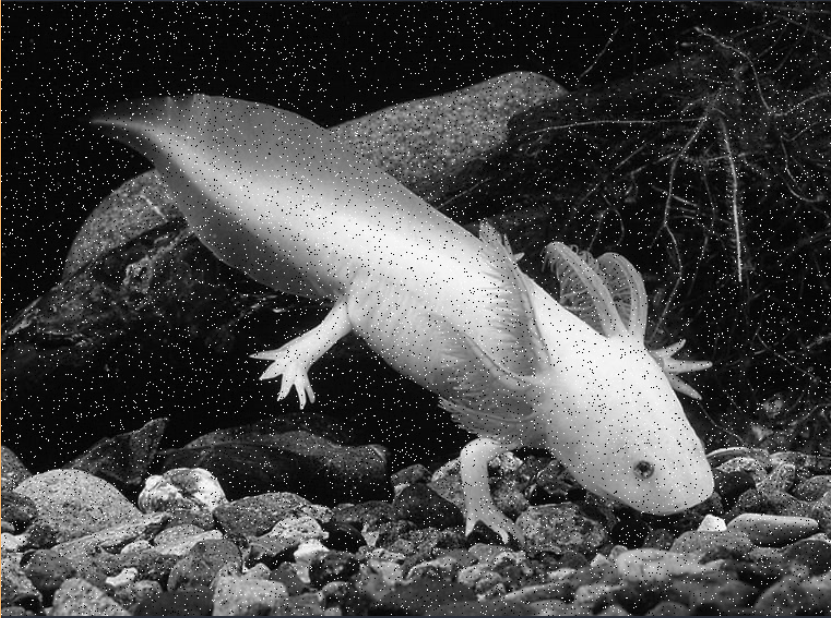
\includegraphics[width=11cm]{Imagenes/Ruido_sp_bn_2.png} \\
				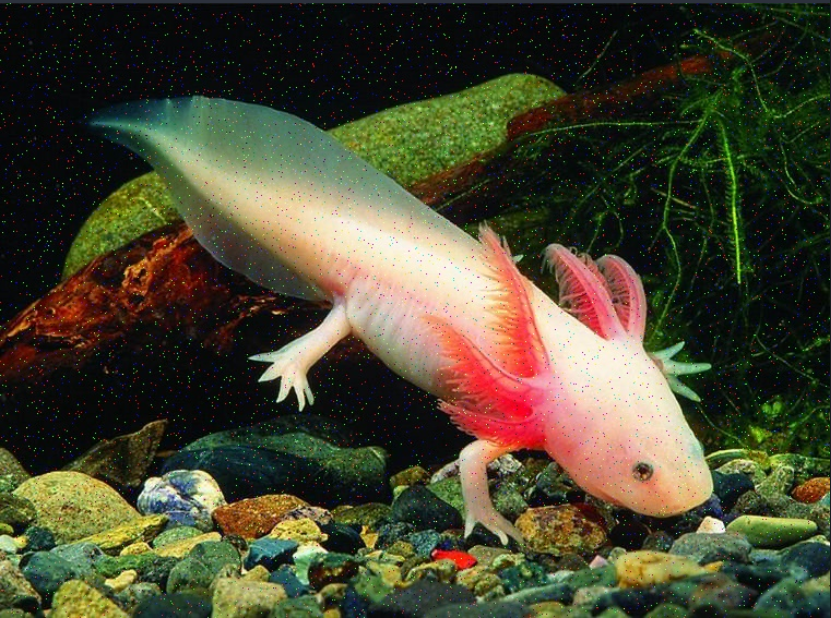
\includegraphics[width=11cm]{Imagenes/Ruido_sp_color_1.png} & 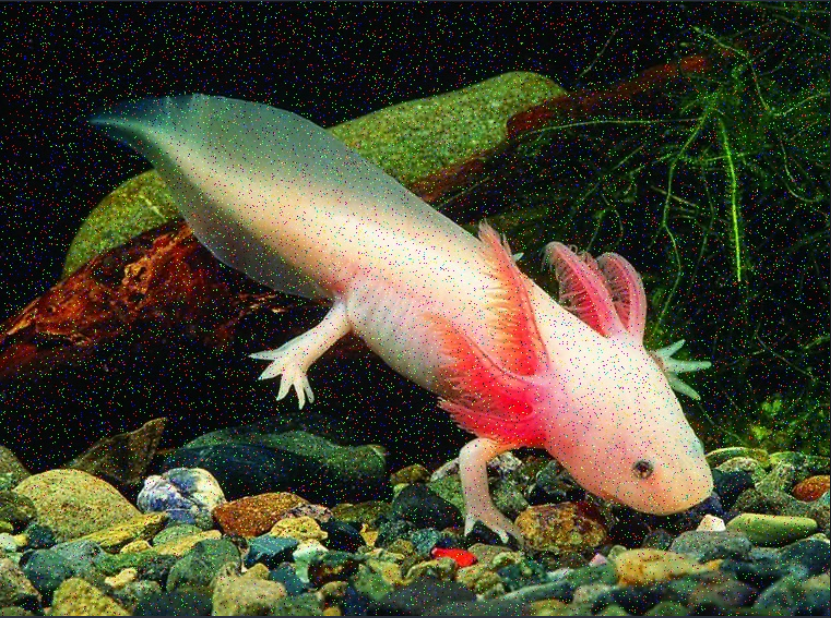
\includegraphics[width=11cm]{Imagenes/Ruido_sp_color_2.png}
			\end{tabular}
			\label{Ruido_sal_pimienta}
			\caption{Ejemplo de imágenes a escala de grises y a color, con ruido tipo sal y pimienta adicionado \\ 1) Imagen en escala de grises con parámetro $l = 150$ \\ 2) Imagen en escala de grises con parámetro $l = 50$ \\ 3) Imagen a color con parámetro $l = 150$ \\ 4)Imagen a color con parámetro $l = 50$}
		\end{figure}
	\end{landscape}
	
	\begin{lstlisting}[language=Python]
		def noise(noise_type:str,image,**kargs):
			list_keys = list(kargs)
			image = copy(image)
			
			if noise_type == "gaussian":
				# Obtains the values of the mean and standard deviation
				mean = kargs['mean'] if 'mean' in list_keys else 0; std_deviation = kargs['std_deviation'] if 'std_deviation' in kargs.keys() else 0.1
				print('mean >>',mean,'  std deviation >>',std_deviation)
				# Creates the noise in a random manner according to the normal distribution with the given mean and standard deviation
				gauss = random.normal(mean,std_deviation,image.shape)
				# The noise gets added
				noisy_image = image + gauss
				# Rectifies that values an the upper and lower limit do not exceeds 0-255
				noisy_image[noisy_image > 255] = 255; noisy_image[noisy_image < 0] = 0
				return noisy_image.astype(uint8)
			elif noise_type == "s&p":
				l = 101 if 'l' not in list_keys else kargs['l']
				# Convert the image to 0 to 1 float to avoid wrapping that occurs with uint8
				image.astype(float16, copy = False)
				image = multiply(image, (1/255))
				# Generate noise to be added to the image
				noise = random.randint(l, size=image.shape)
				# Convert high and low bounds of l in noise to salt and pepper noise then add it to
				# our image. 1 is subtracted from l to match bounds behaviour of random.randint.
				image = where(noise == 0, 0, image)
				image = where(noise == (l-1), 1, image)
				# Properly handles the conversion from float16 back to uint8
				image = cv2.convertScaleAbs(image, alpha = (255/1))        
				return image
	\end{lstlisting}
	
	\hfill\break
	\justifying
	La implementación del ruido gausiano es bastante sencilla y muy conveniente si se apoya de la herramienta que provee la biblioteca numpy en su módulo random. La función \textit{normal}, genera un array con valores tomados de forma aleatoria de una distribución normal con una cierta media y desviación estándar dada para una cierta dimensionalidad.
	
	\hfill\break
	\justifying
	Lo que resta una vez creados estos valores, es realizar la suma elemento por elemento con la imagen, y con esta acción se ha adicionado el ruido con distribución gausiana. Importante la penúltima instrucción que va a rectificar aquellos valores en la nueva imagen con ruido, que excedan los límites superiores(255) e inferior(0).
	
	\hfill\break
	\justifying
	Finalmente la adición del ruido sal y pimienta inicia convirtiendo el arreglo de la imagen en valores enteros a un tipo de dato float y se realiza la normalización, esto para evitar errores en la asignación de los nuevos valores.
	
	\hfill\break
	\justifying
	Al igual que sucede con el ruido gausiano, el trabajo se auxilia de la herramienta aleatoria disponible en numpy que permite generar un arreglo de tamaño igual al número de elementos en la imagen, definiendo el número más alto que puede tomarse y simplemente se asigna al pixel el valor 0 cuando en el mismo índice el arreglo del ruido tiene el valor 0. De forma similar, cuando el indice del arreglo de ruido tiene el valor del límite especificado menos 1, la imagen toma el valor saturado en ese pixel.
	
	\hfill\break
	\justifying
	Resta únicamente escalar de vuelta los valores del rango 0.0-1.0 a 0-255, y se retorna la imagen adicionada con ruido.
	
\newpage

\section*{4. Filtrado de imagen}
	\hfill\break
\justifying
Como siguiente sección se colocan las funciones de filtrado. Los filtros son herramientas utilizadas para ayudar a eliminar o suavizar los efectos que tiene el ruido en una imagen.

\hfill\break
\justifying
Existen filtros que operan en el espectro frecuencial, otros en el espacial, etc. La clasificación que interesa en este trabajo será la de los filtros lineales y no lineales en el dominio espacial de los pixeles.

\hfill\break
\justifying
Los filtros en las imágenes pueden utilizarse para recorrer espectralmente la señal que interesa, consiguiéndose con la ayuda de un \textit{kernel}, que es simplemente una matriz pequeña que es convolucionada con la imagen para ejecutar un filtro adecuado.

\hfill\break
\justifying
Para los filtros que fueron implementados en el trabajo, se define siempre un \textit{kernel}, que se deja como un parámetro modificable por el usuario, pues la importancia que tiene el tamaño de este en el espectro de las frecuencias, equivaldría a modificar en un filtro analógico la frecuencia de corte.

\subsection*{Filtros lineales}
	
	\subsubsection*{Filtrado Promedio Aritmético}
		\hfill\break
		\justifying
		Considerado en la clasificación de filtros lineales, este tipo de filtro, ocupa un \textit{kernel} con valores unitarios en sus elementos, y se utiliza para la realización de la convolusión entre una ventana de la imagen y el \textit{kernel}.
		
		\hfill\break
		\justifying
		Esta convolusión resulta simplemente en la suma de todos los valores en esa ventana, aplicándoseles la división entre el número de elementos en la ventana y obteníendose el valor promedio que será asignado como nuevo valor al elemento ancla o central de la ventana.
		
		\begin{equation*}
			f_{pa} = \frac{1}{n^2} \sum_{(x,y)\in V} f(x,y)
		\end{equation*}
	
		La aplicación del filtro resulta visualmente en el desenfoque de la imagen, lo que se interpreta como el filtrado de las frecuencias más altas conservando aquellas más bajas.
		
	\subsubsection*{Filtro Gaussiano}
		\hfill\break
		\justifying
		El filtro gaussiano matemáticamente se define por la modificación de una señal de entrada por medio de una convolución con una función gausiana.
		
		\hfill\break
		\justifying
		Considerado el filtro ideal en el dominio del tiempo, tienen la propiedad de no sobrepasar la entrada de una función escalonada y al mismo tiempo disminuir el tiempo de subida y bajada.
		
		\hfill\break
		\justifying
		En el procesamiento de imágenes, cada elemento de la matriz representa un atributo de píxel, como el brillo o la intensidad del color, y el efecto generl que se obtiene de su implementación se le denomina desenfoque gaussiano.
		
		
	\begin{landscape}
		\hfill\break
		\hfill\break
		\hfill\break
		\begin{figure}[!h]
			\begin{tabular}{cc}
				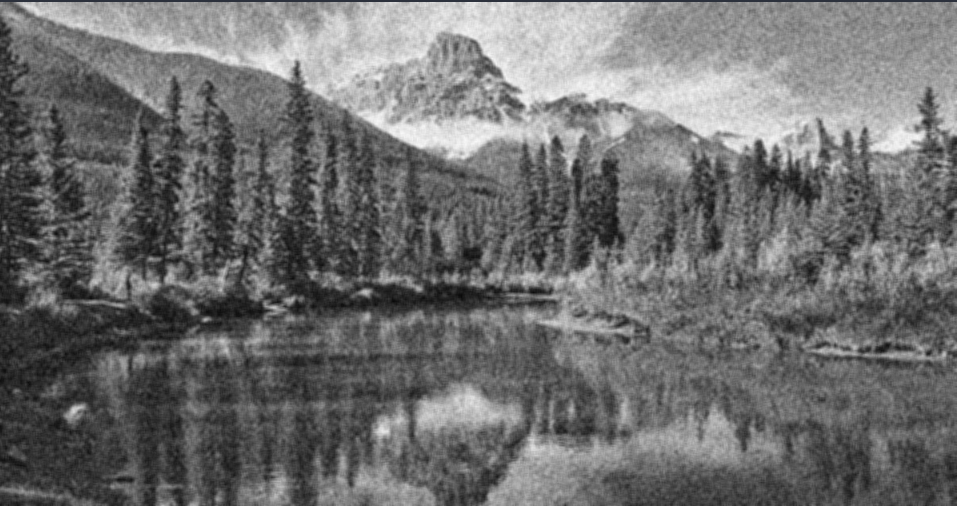
\includegraphics[width=12.25cm]{Imagenes/Ruido_Gauss_5_50_FMA_5.png} & 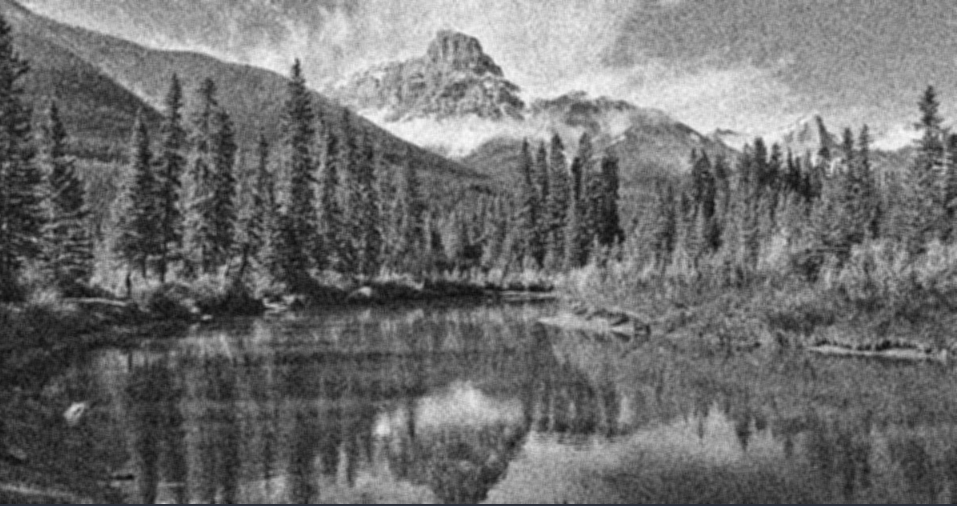
\includegraphics[width=12.25cm]{Imagenes/Ruido_Gauss_5_50_Gauss_5_5.png} \\
				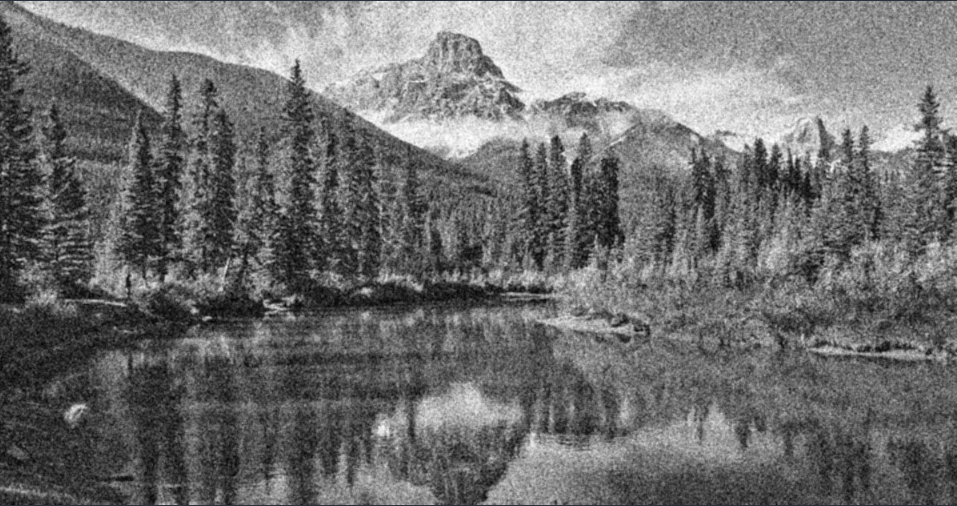
\includegraphics[width=12.25cm]{Imagenes/Ruido_Gauss_5_50_FMA_3.png} & 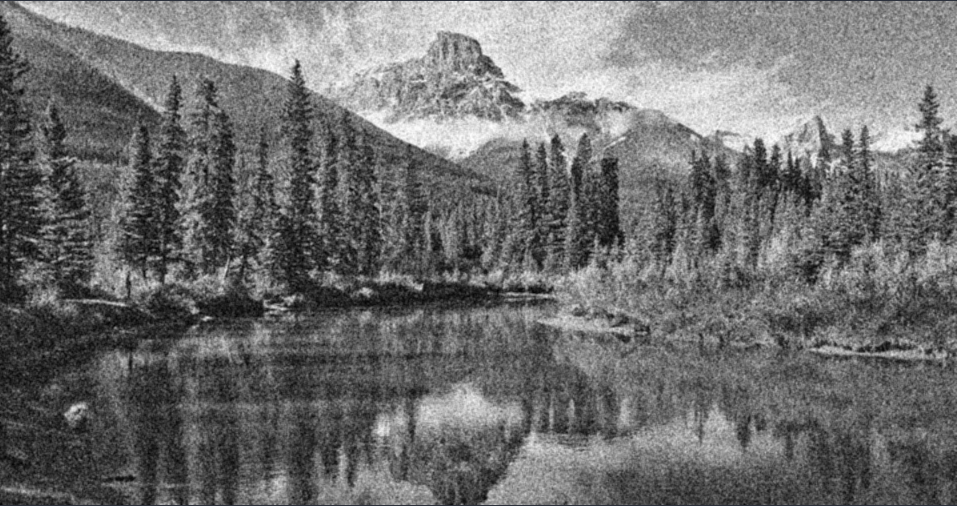
\includegraphics[width=12.25cm]{Imagenes/Ruido_Gauss_5_50_Gauss_5_3.png}
			\end{tabular}
			\label{Ruido_Gauss_Filtros_lineales}
			\caption{Ejemplo de imágenes adicionadas con ruido Gaussiano con $\mu = 5$ y $\sigma = 50$ y los filtros lineales. \\ 1) Imagen filtrada con el Filtro Media Aritmética y tamaño de \textit{kernel} $n = 5$ \\ 2) Imagen filtrada utilizando el Filtro Gaussiano con parámetros $\sigma = 5$ y tamaño de \textit{kernel} $n = 5$ \\ 3) Imagen filtrada con el Filtro Media Aritmética y tamaño de \textit{kernel} $n = 3$ \\ 4)Imagen filtrada utilizando el Filtro Gaussiano con parámetros $\sigma = 5$ y tamaño de \textit{kernel} $n = 3$}
		\end{figure}
		
		\newpage
		
		\begin{figure}[!h]
			\begin{tabular}{cc}
				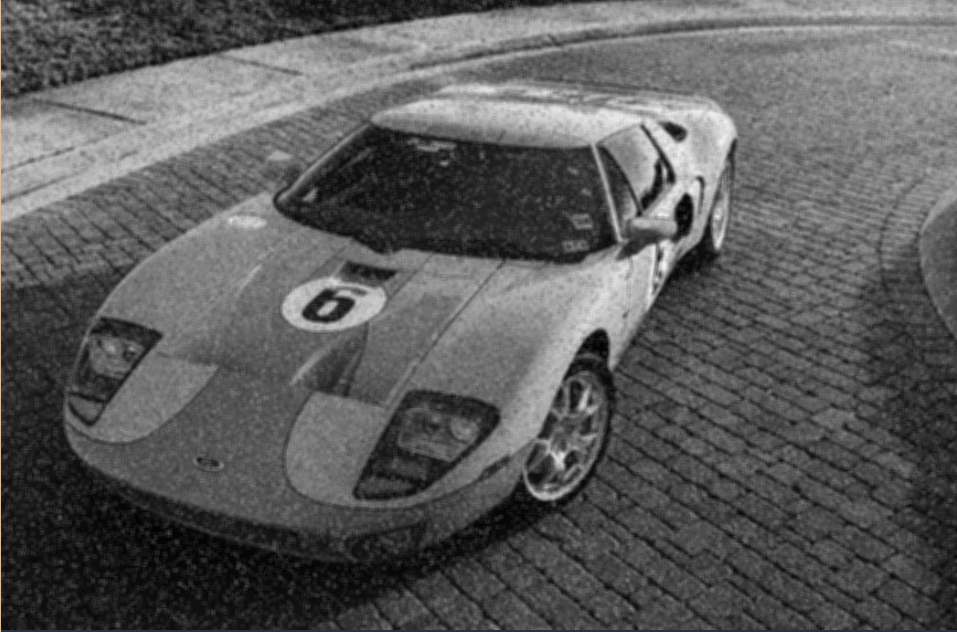
\includegraphics[width=12.25cm]{Imagenes/Ruido_sp_25_FMA_5.png} & 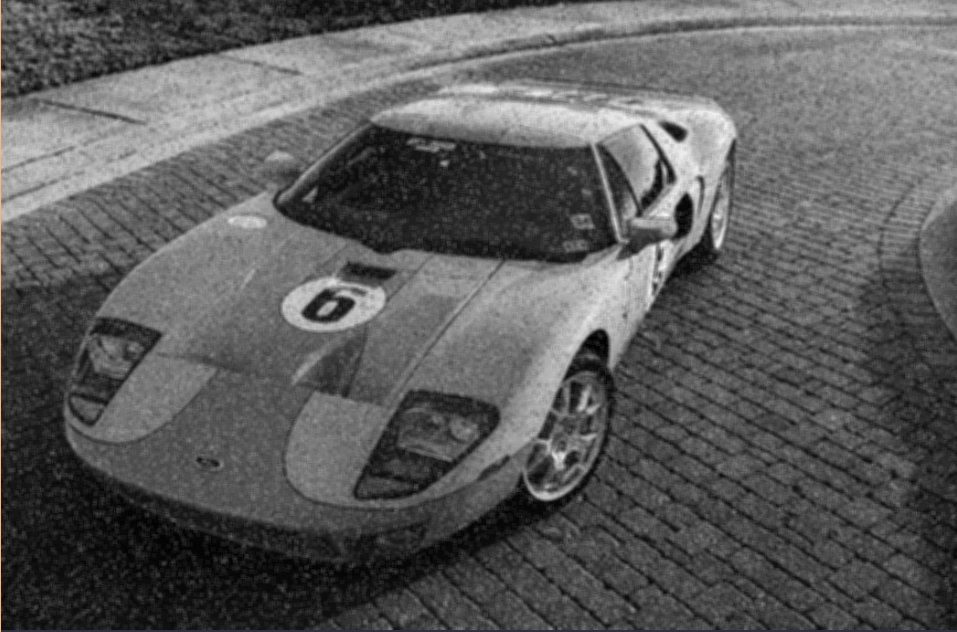
\includegraphics[width=12.25cm]{Imagenes/Ruido_sp_25_Gauss_5_5.png} \\
				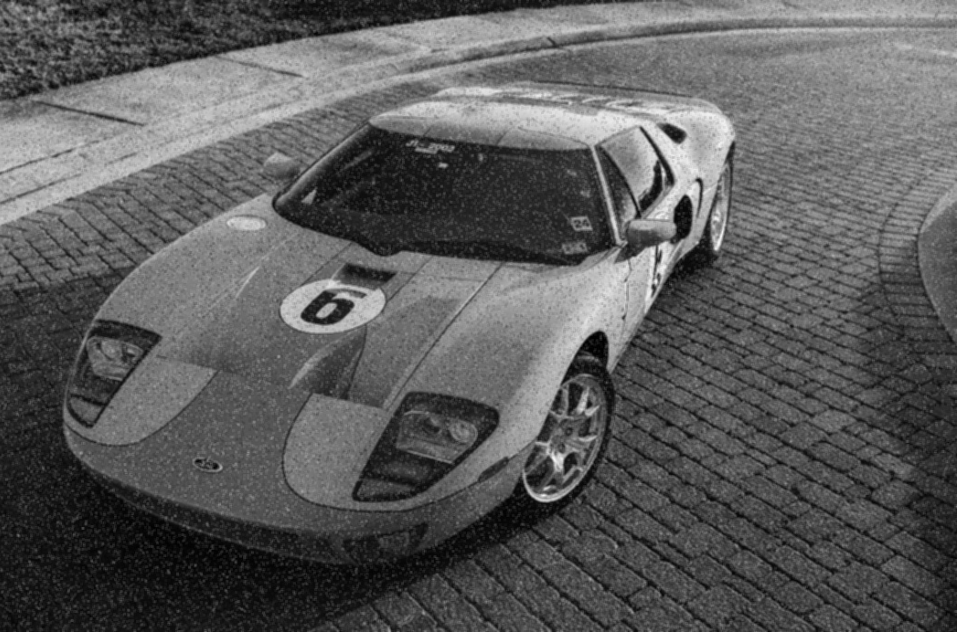
\includegraphics[width=12.25cm]{Imagenes/Ruido_sp_25_FMA_3.png} & 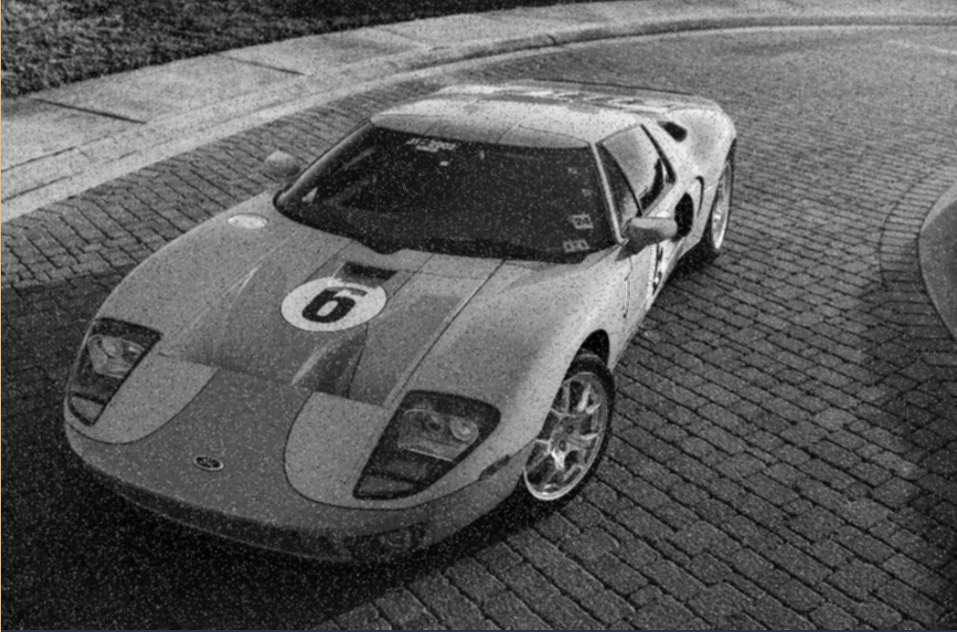
\includegraphics[width=12.25cm]{Imagenes/Ruido_sp_25_Gauss_5_3.png}
			\end{tabular}
			\label{Ruido_SalPimienta_Filtros_lineales}
			\caption{Ejemplo de imágenes adicionadas con ruido Sal y Pimienta, con $l = 25$ y los filtros lineales. \\ 1) Imagen filtrada con el Filtro Media Aritmética y tamaño de \textit{kernel} $n = 5$ \\ 2) Imagen filtrada utilizando el Filtro Gaussiano con parámetros $\sigma = 5$ y tamaño de \textit{kernel} $n = 5$ \\ 3) Imagen filtrada con el Filtro Media Aritmética y tamaño de \textit{kernel} $n = 3$ \\ 4)Imagen filtrada utilizando el Filtro Gaussiano con parámetros $\sigma = 5$ y tamaño de \textit{kernel} $n = 3$}
		\end{figure}
	\end{landscape}

	\subsection*{Filtros no lineales}
		\hfill\break
		\justifying
		Un filtro no lineal es aquel cuya salida no es una función lineal de su entrada. Este tipo de filtros suelen tener muchas aplicaciones especialmente en ruidos no aditivos.
		
		\hfill\break
		\justifying
		En comparación con los filtros lineales, estos tienen un comportamiento muy distinto, siendo la características más importante para estos, la salida del filtro o la respuesta del filtro no obedece a principios como la escala y la invarianza. Este tipo de filtros pueden producir resultados que varian de una manera no intuitiva.
		
		\hfill\break
		\justifying
		El principio general de operación de los filtros no lineales de orden es:
		\begin{enumerate}
			\item Ordenamiento de los valores dentro de la ventana de valore desordenados
			\item Elegir una regla para la selección de algún valor
			\item Asignación del el nuevo valor en la imagen de salida
		\end{enumerate}
	
		\subsubsection*{Filtro Mediana}
			\hfill\break
			\justifying
			Este filtro tiene un comportamiento muy sencillo, que equivale a ordenar los valores dentro de la ventana en forma ascedente, y tomar como nuevo valor del elemento central el elemento mediano de la secuencia.
			
			\hfill\break
			\justifying
			Suelen obtener buenos resultados para imágenes con ruido Sal y Pimienta.
			
		\subsubsection{Filtros Max y Min}
			\hfill\break
			\justifying
			Iniciando con el mismo proceso, se ordena la secuencia en forma ascendente y se toman los valores extremos en cada filtro. Para el filtro Max, se toma el último valor, el más grande, mientras que para el filtro Min el primero.
		
		\begin{figure}[!h]
			\begin{tabular}{cc}
				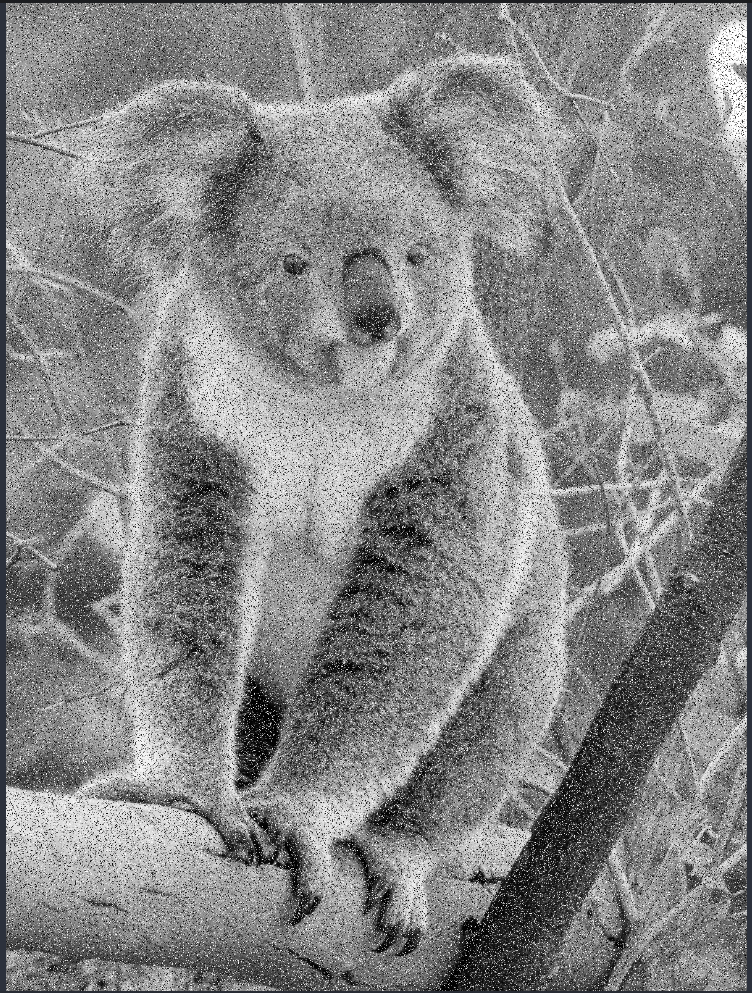
\includegraphics[width=8.5cm]{Imagenes/Ruido_sp_10_.png} & 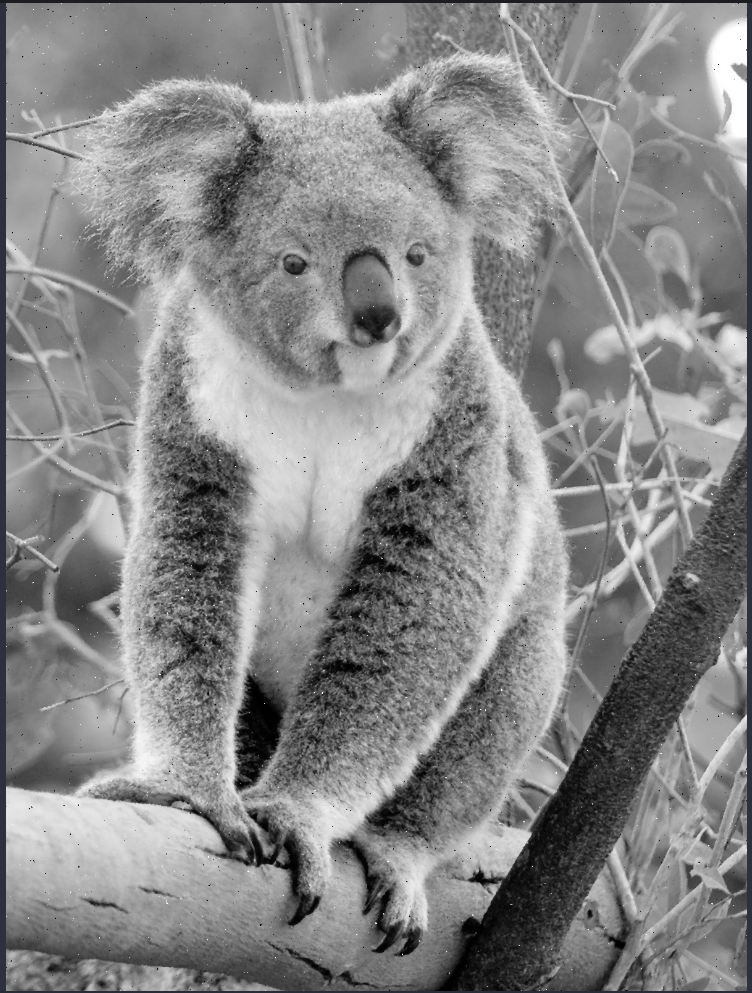
\includegraphics[width=8.5cm]{Imagenes/Ruido_sp_10_mediana_3.png} \\
			\end{tabular}
			\label{Ruido_SP_Filtro_no_lineale_mediana}
			\caption{Ejemplo de una imágene adicionada con una gran cantidad de ruido Sal y Pimienta con $l = 10$ y más sin embargo con el uso del filtro mediano con \textit{kernel} tamaño $n=3$ se logra eliminar una gran cantidad de ruido}
		\end{figure}
		
	\begin{landscape}
		\hfill\break
		\hfill\break
		\hfill\break
		\hfill\break
		\begin{figure}[!h]
			\centering
			\begin{tabular}{ccc}
				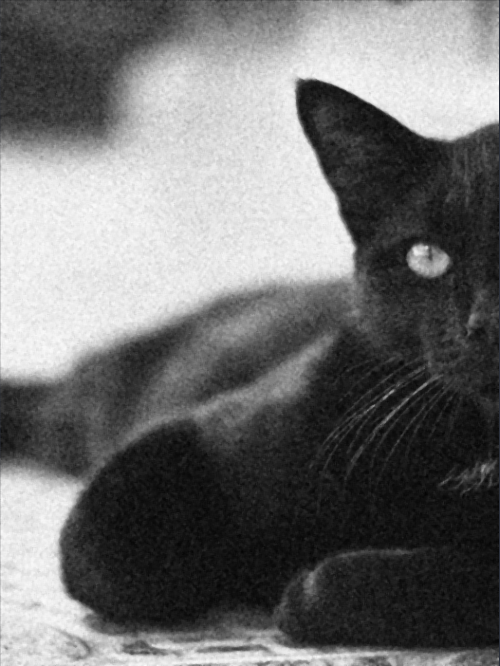
\includegraphics[width=8cm]{Imagenes/Ruido_Gauss_5_50_mediana_5.png} & 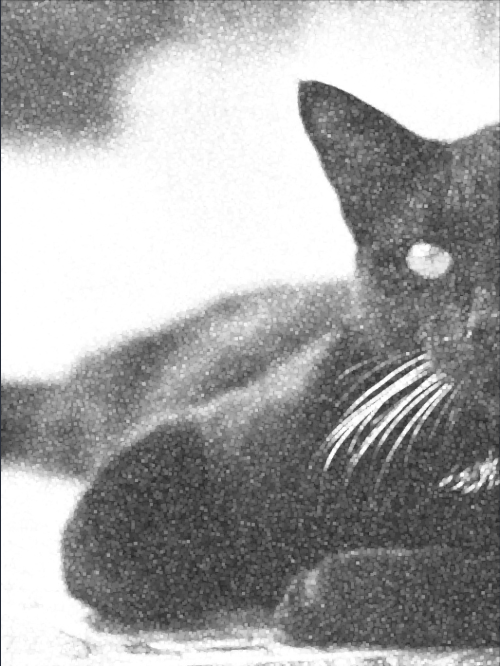
\includegraphics[width=8cm]{Imagenes/Ruido_Gauss_5_50_max_5.png} &
				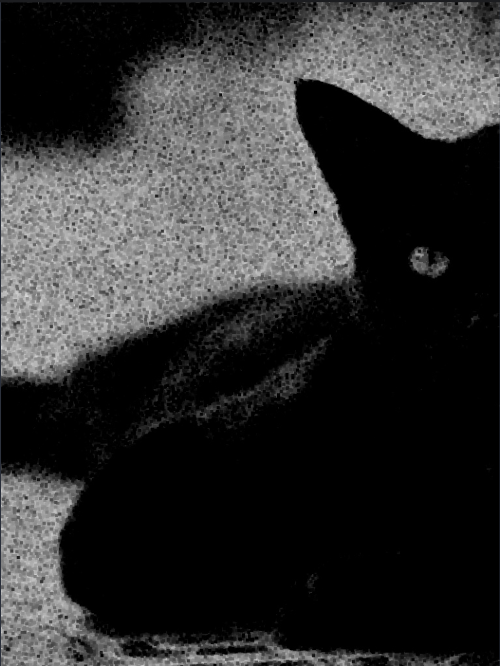
\includegraphics[width=8cm]{Imagenes/Ruido_Gauss_5_50_min_5.png}
			\end{tabular}
			\label{Ruido_Gauss_Filtros_no_lineales}
			\caption{Ejemplo de imágenes adicionadas con ruido Gaussiano con $\mu = 5$ y $\sigma = 50$ y los filtros no lineales de orden. \\ 1) Imagen filtrada con el Filtro Mediana con tamaño de \textit{kernel} $n = 5$ \\ 2) Imagen filtrada utilizando el Filtro Max con tamaño de \textit{kernel} $n = 5$ \\ 3) Imagen filtrada con el Filtro Min con tamaño de \textit{kernel} $n = 5$ }
		\end{figure}
	
		\newpage
		
		\begin{figure}[!h]
			\begin{tabular}{cc}
				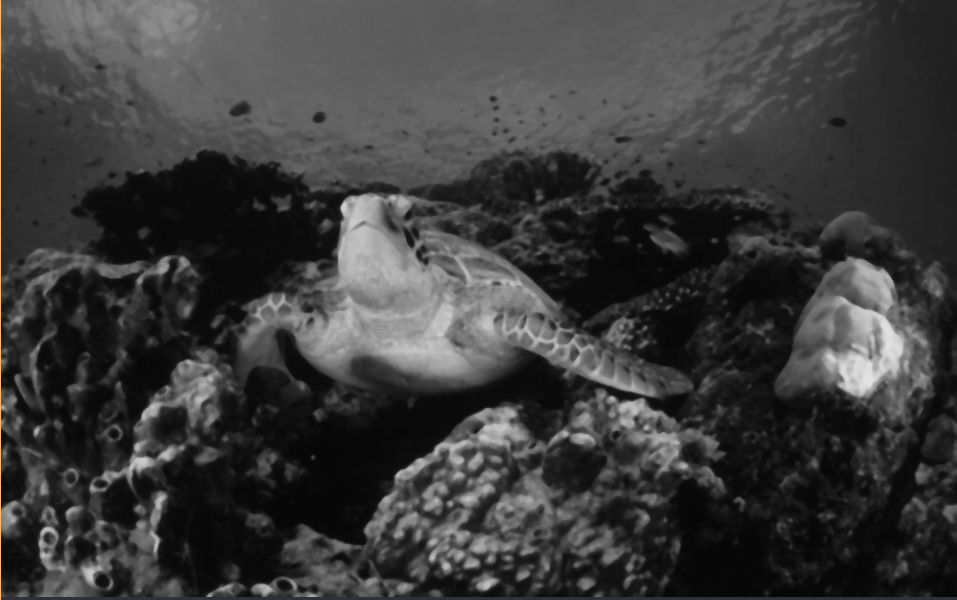
\includegraphics[width=12.25cm]{Imagenes/Ruido_sp_50_mediana_5.png} & 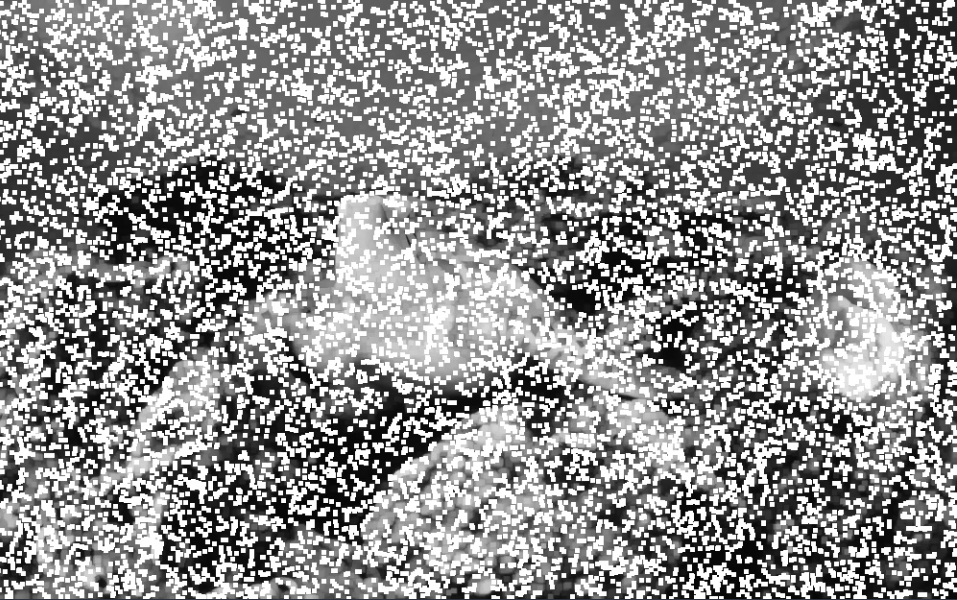
\includegraphics[width=12.25cm]{Imagenes/Ruido_sp_50_max_5.png} \\
				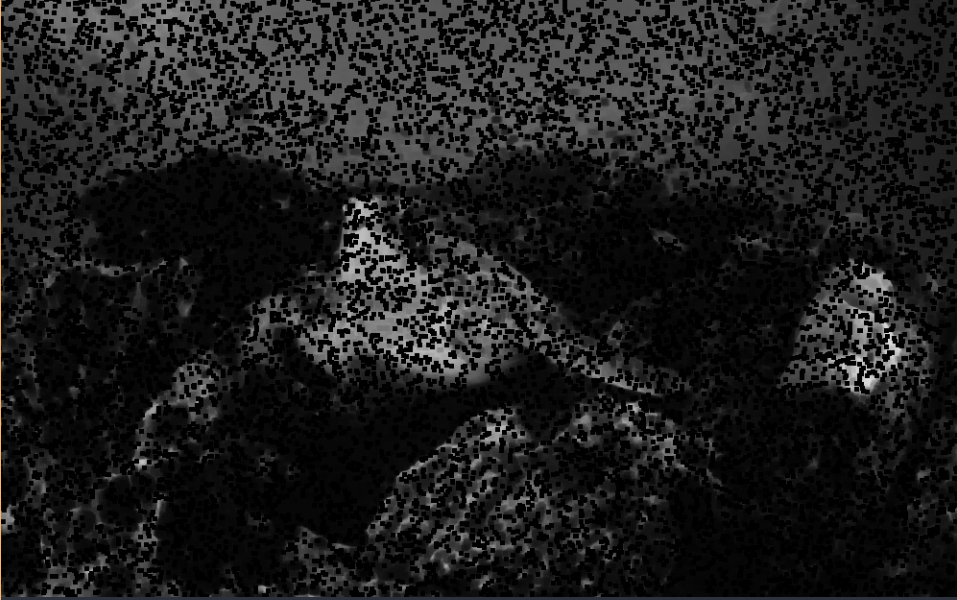
\includegraphics[width=12.25cm]{Imagenes/Ruido_sp_50_min_5.png} & 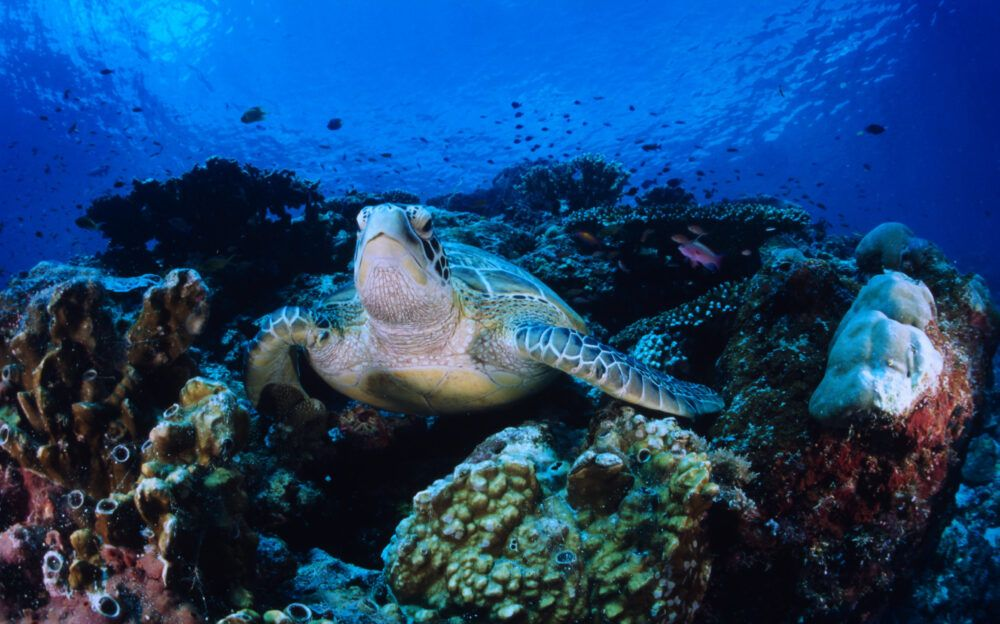
\includegraphics[width=12.25cm]{Imagenes/tortuga.jpeg}
			\end{tabular}
			\label{Ruido_SalPimienta_Filtros_no_lineales}
			\caption{Ejemplo de imágenes adicionadas con ruido Sal y Pimienta, con $l = 50$ y los filtros no lineales de orden. \\ 1) Imagen filtrada con el Filtro Mediana con tamaño de \textit{kernel} $n = 5$ \\ 2) Imagen filtrada utilizando el Filtro Max con tamaño de \textit{kernel} $n = 5$ \\ 3) Imagen filtrada con el Filtro Min con tamaño de \textit{kernel} $n = 5$ \\ 4) Fotografía original de tortuga nadando entre arrecifes. }
		\end{figure}
	\end{landscape}

	\begin{lstlisting}[language=Python]
		def filtering(filter_type:str,image,n:int=3,**kargs):
			image = copy(image)
			
			if filter_type == 'mean':
				# Kernel creation
				#   Before applying any convolution with an image using a 2D matrix it's needed to ensure 
				#   all the values are normalize, thus the division of the matrix
				kernel = ones((n,n),float32)/(n**2)
				# Mean filtering
				#   ddepth: a -1 value means the final image will also have the same depth as the original
				return cv2.filter2D(image,-1,kernel)
			elif filter_type == 'gaussian':
				std_deviation = 0 if 'std_deviation' not in list(kargs) else kargs['std_deviation']
				return cv2.GaussianBlur(image,(n,n),std_deviation)
			elif filter_type == 'median':
				return cv2.medianBlur(image,n)
			elif filter_type == 'max':
				# The morphological dilation is equivalent to a maximum filter
				kernel = cv2.getStructuringElement(cv2.MORPH_RECT,(n,n))
				return cv2.dilate(image,kernel)
			elif filter_type == 'min':
				# The morphological erosion is equivalent to a minimum filter
				kernel = cv2.getStructuringElement(cv2.MORPH_RECT,(n,n))
				return cv2.erode(image,kernel)
	\end{lstlisting}
	
\newpage
	
\section*{5. Operaciones Morfológicas}
	\hfill\break
\justifying
Como penúltima sección se tienen a las operaciones morfológicas. Del área de estudio Morfología Matemática desarrollada por los hermanos Minkosky, la idea básica detrás de la Morfología Matemática es probar una imagen pormedio de un probador, que se denomina Elemento de Estructura(EE), y cualificar de esta manera en que dicho EE encaja, o no, una imagen.

\hfill\break
\justifying
Ayudándose del marcado de los EE que si encajan en un objeto, uno es capaz de derivar información relacionada con la estructura relativa a la imagen y el objeto.

\hfill\break
\justifying
La información que se obtenga dependerá del tamaño del EE así como de su forma, siendo de gran importancia la elección de un EE correcto.

\hfill\break
\justifying
Dos operaciones dentro de la teoría de la Matemática Morfológica son escenciales, y es que son la base de la derivación de las demás operaciones:

\subsection*{Operaciones básicas}
	\subsubsection*{Erosión}
		\hfill\break
		\justifying
		\textbf{Formalmente}: Sean \textit{A} y \textit{B} 2 conjuntos en $Z^2$, la erosión de \textit{A} por \textit{B} denotada como $A\Theta B$ se define como:
		\begin{equation*}
			A\Theta B = {x|(B)_x\subseteq A}
		\end{equation*}
	
		\hfill\break
		\justifying
		En otras palabras, la erosión de \textit{A} por \textit{B} es el conjunto de todos los puntos \textit{x} tal que \textbf{B} trasladada por \textit{x} está contenida en \textit{A}.
		
		\hfill\break
		\justifying
		Visualmente el resultado que se obtiene de aplicar una erosión es el adelgazamiento de la figura en la que se aplica, esto por supuesto, influenciado por la forma de la estructura EE.
		
	\subsubsection*{Dilatación}
		\hfill\break
		\justifying
		\textbf{Formalmente:} Sean \textit{A} y \textit{B} 2 conjuntos en $Z^2$, la dilatación de \textit{A} por \textit{B}, denotada como $A\oplus B$ se define como:
		\begin{equation*}
			A\oplus B = {x|\hat{B_x} \cap A \neq \oslash}
		\end{equation*}
	
		\hfill\break
		\justifying
		En otras palabras, el proceso de dilatación consiste en obtener la reflexión del elemento estrsucturante \textit{B} al rededor de su origen y después desplazar esta reflexión por \textit{x}. $A\oplus B$ es entonces el conjunto de todos los desplazamientos en \textit{x} tales que $\hat{B}$ y \textit{A} comparten al menos un elemento no igual al cero.
		
		\hfill\break
		\justifying
		Visualmente después de aplicar la dilatación sobre un objeto este se notará más ensanchado. La capacidad de que el objeto conserve su forma original dependerá de la elección del EE y su tamaño.

\subsubsection*{Operaciones derivadas}
	\hfill\break
	\justifying
	Con el objeto de aumentar el efecto de las operaciones básicas, se pueden diseñar filtros consistentes ne la iteración de varias operaciones de erosión o de dilatación.
	
	\hfill\break
	\justifying
	En ocasiones la aplicación de 1 sola iteración de operaciones no da el resultado esperado, por lo que es necesario el encadenamiento de n iteraciones de filtrado para obtener el resultado.
	
	\hfill\break
	\justifying
	El uso de las operaciones básicas en conjunto es común en este tipo de iteraciones, y sin embargo es fácil pensar que las operaciones de dilatación y erosión son opuesta, pero es en general no es cierto, de forma que implementación conjunta da apertura a nuevas operaciones.
	
	\subsubsection*{Apertura Morfológica}
		\hfill\break
		\justifying
		\textbf{Formalmente:} Sean \textit{A} y \textit{B} dos conjuntos en $Z^2$, la apertura de \textit{A} por \textit{B}, denotada como $A \circ B$ se define como:
		\begin{equation*}
			A \circ B = (A\Theta B) \oplus B
		\end{equation*}
	
		\hfill\break
		\justifying
		En otras palabras, la apertura de \textit{A} por \textit{B} es simplemente y sencillamente la erosión de \textit{A} por \textit{B} seguida de la dilatación del resultado.
		
	\subsubsection*{Cerradura Morfológica}
		\hfill\break
		\justifying
		\textbf{Formalmente:} Sean \textit{A} y \textbf{B} dos conjuntos en $Z^2$, la cerradura de \textit{A} por \textit{B}, denotada como $A \bullet B$, se define como:
		\begin{equation*}
			A\bullet B = (A\oplus B)\Theta B
		\end{equation*}
	
		\hfill\break
		\justifying
		En otras palabras, la cerradura de \textit{A} por \textbf{B} es simple y sencillamente la dilatación de \textit{A} por \textbf{B} seguida de la erosión del resultado.

\subsubsection{Implementación}
	\hfill\break
	\justifying
	A continuación se ejemplifica el poder de las operaciones morfológicas en una situación donde se cuenta con una imagen de monedas que pueden ser contadas con el algoritmo básico de \textbf{bit-quad}, sin embargo la sola binarización con un umbral no da un resultado para implementarlo, de forma que aplicando en cadena las operaciones se consigue limpiar perfectamente la imagen binarizada para aplicar en el algoritmo de contabilización de objetos.
	
	\begin{figure}[!h]
		\centering
		\begin{tabular}{cc}
			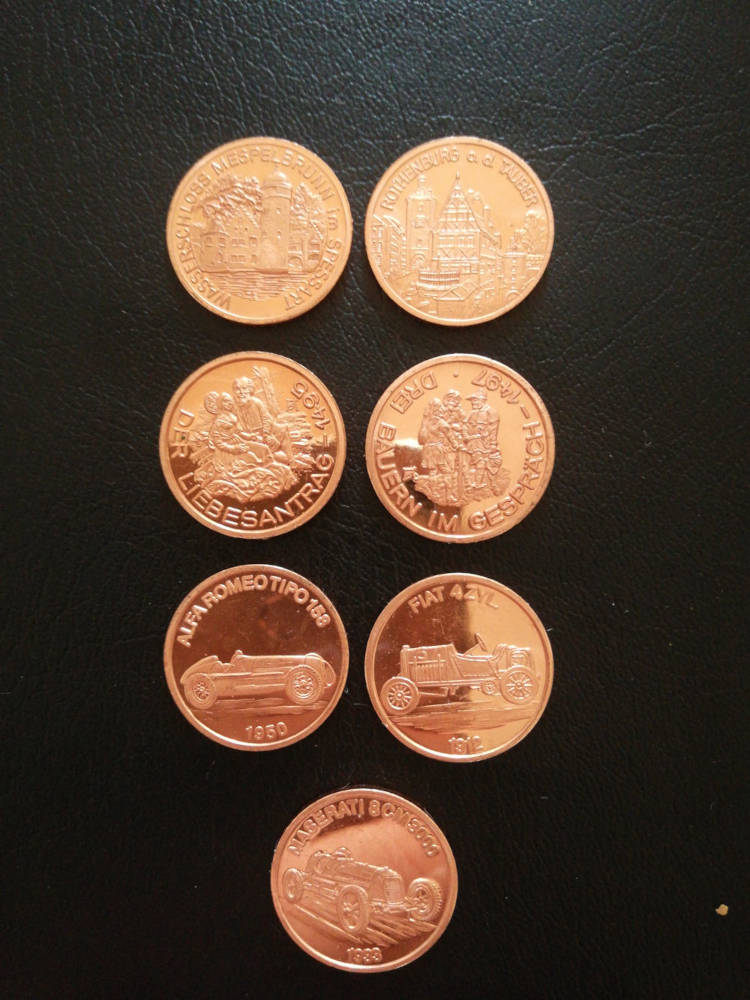
\includegraphics[width=7.5cm]{Imagenes/monedas_2_chica.jpeg} & 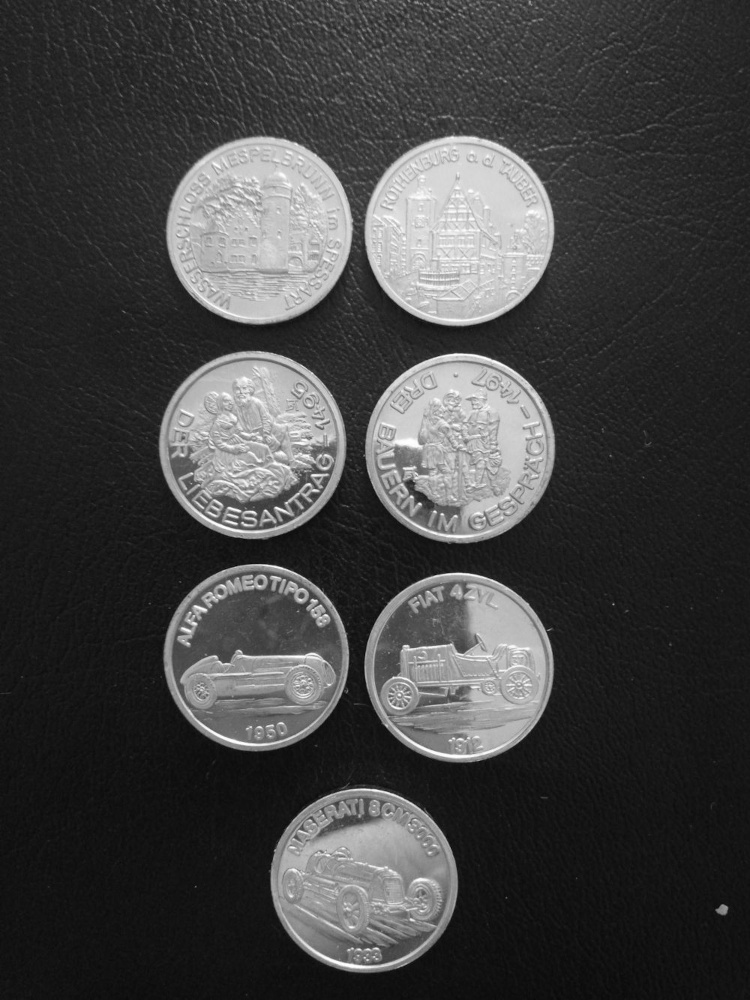
\includegraphics[width=7.5cm]{Imagenes/op_morf_monedas_0.jpeg}
		\end{tabular}
		\caption{1) Imagen original de las monedas. Colocadas sobre un fondo obscuro con gran contraste, nos enfrentamos a la textura tipo vinil que con la iluminación no es completamente negro \\ 2) Transformación a escala de grises de la imagen original}
	\end{figure}

	\newpage

	\begin{figure}[!h]
		\centering
		\begin{tabular}{cc}
			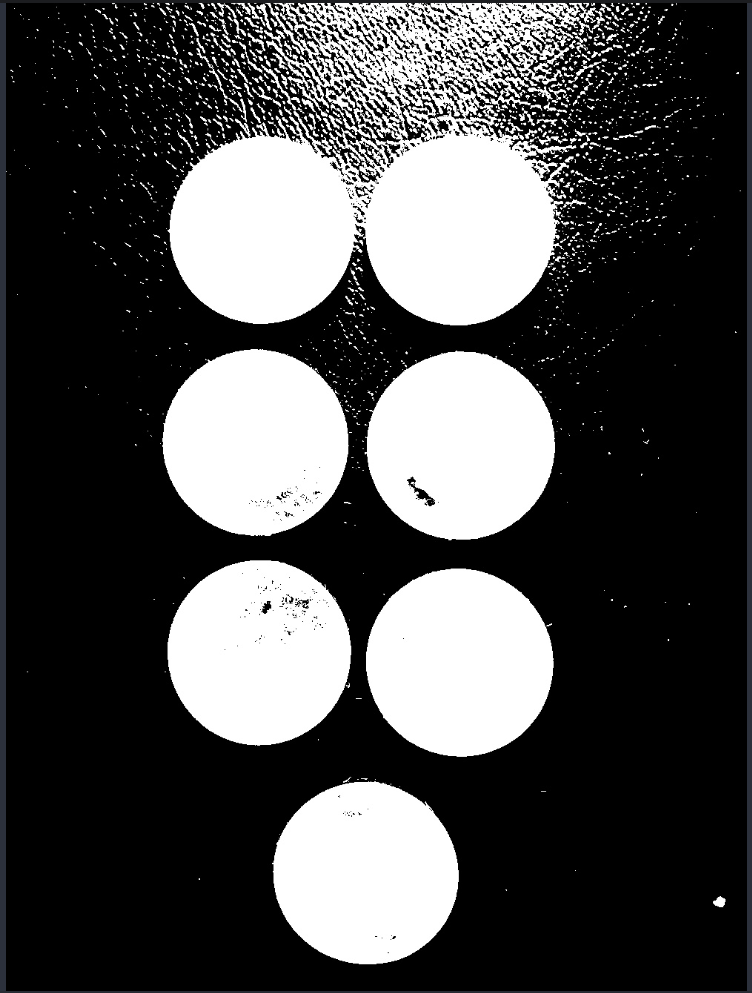
\includegraphics[width=7.5cm]{Imagenes/op_morf_monedas_1.png} & 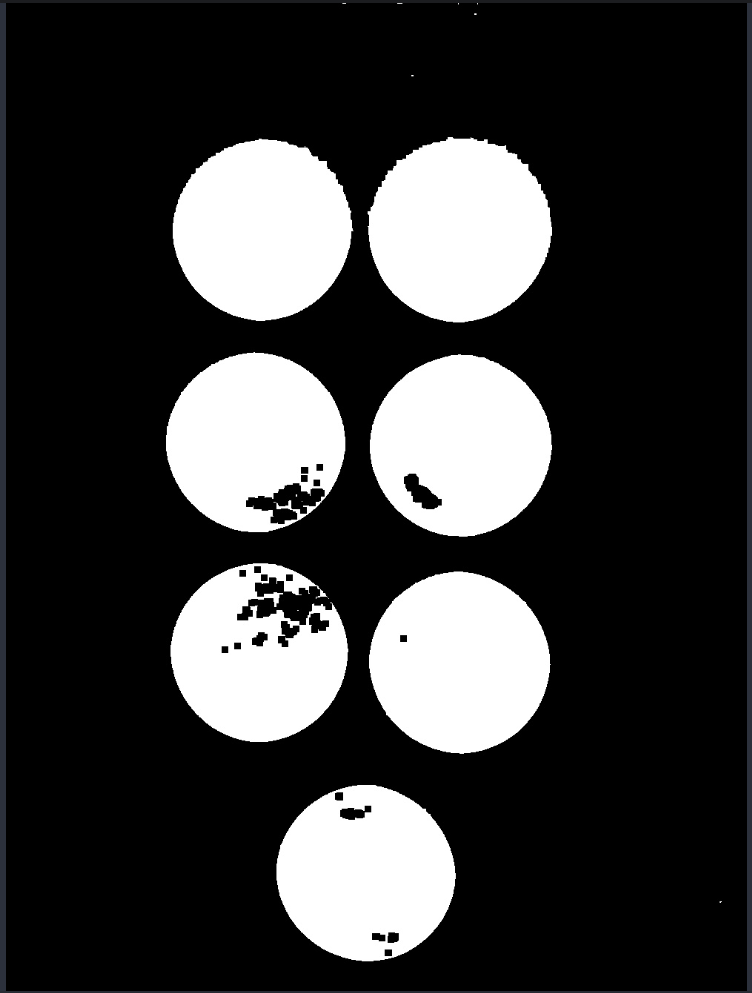
\includegraphics[width=7.5cm]{Imagenes/op_morf_monedas_2.png} \\
			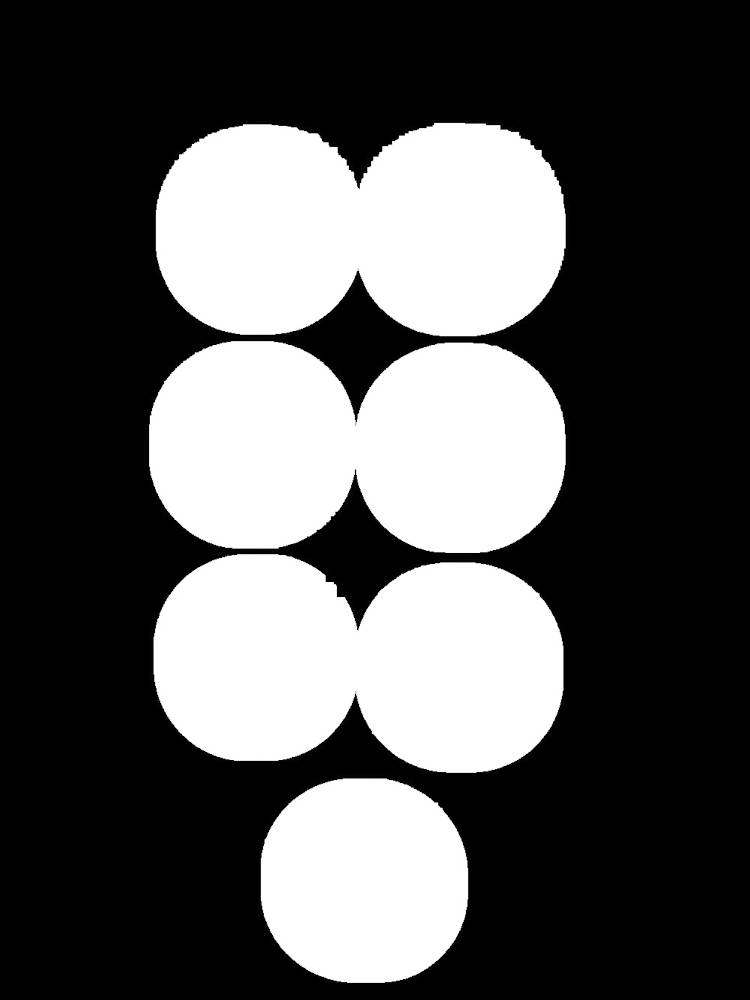
\includegraphics[width=7.5cm]{Imagenes/op_morf_monedas_3.jpeg} & 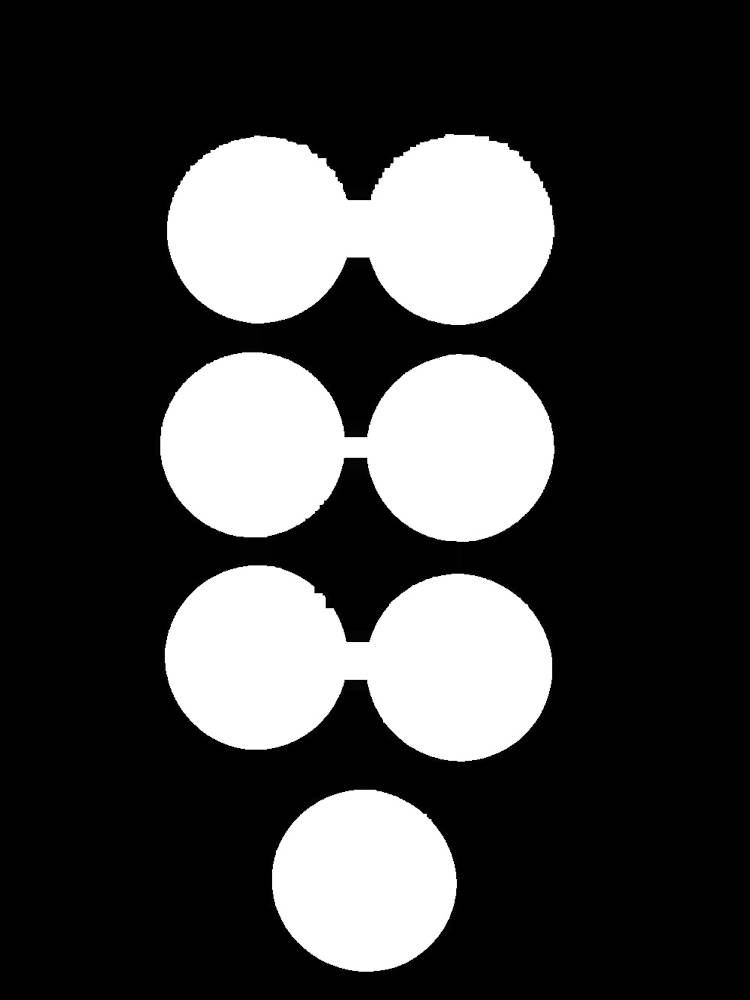
\includegraphics[width=7.5cm]{Imagenes/op_morf_monedas_4.jpeg} 
		\end{tabular}
		\caption{1) Binarización de la imagen con un umbral manual de 60. Se aprecia que debido a la textura en la parte superior la binarización no lo colorea como el fondo\\ 2) Aplicando una operación de erosión con un kernel grande de $n=9$ se elimina casi por completo las textura mal coloreada. Se termina por aplicar una erosión más con un kernel pequeño de $n=3$. \\ 3) Para poder rellenar los espacios en negro dentro las monedas se aplican consecutivamente 3 dilataciones con kernel $n=9$ y 1 dilatación con $n=5$. Se han rellenado las monedas pero se encuentran unidas. \\ 4) Aplicando consecutivamente la erosión con kernel grande de $n=12$ se separan las monedas. }
	\end{figure}

	\newpage

	\begin{figure}[!h]
		\centering
		\begin{tabular}{cc}
			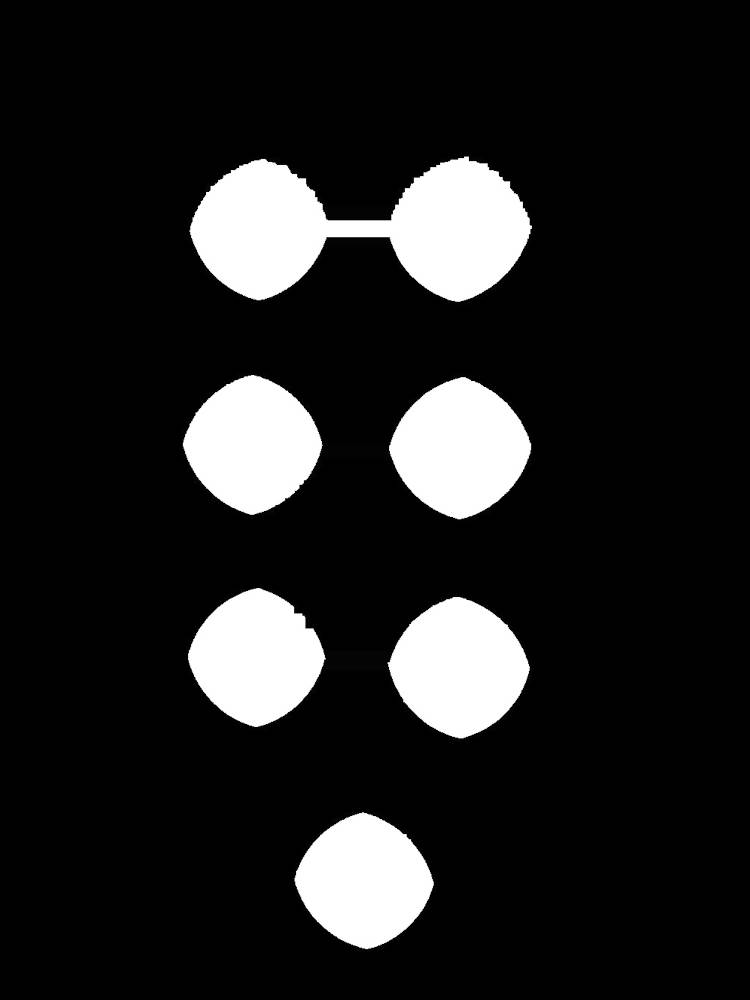
\includegraphics[width=7.5cm]{Imagenes/op_morf_monedas_5.jpeg} & 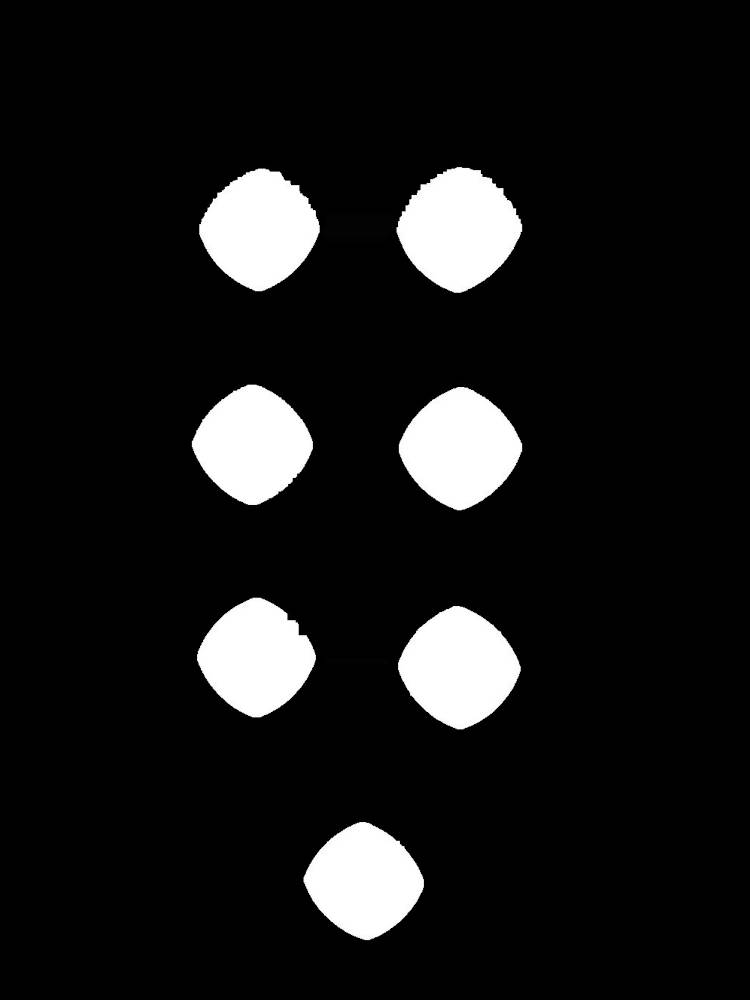
\includegraphics[width=7.5cm]{Imagenes/op_morf_monedas_6.jpeg} \\
			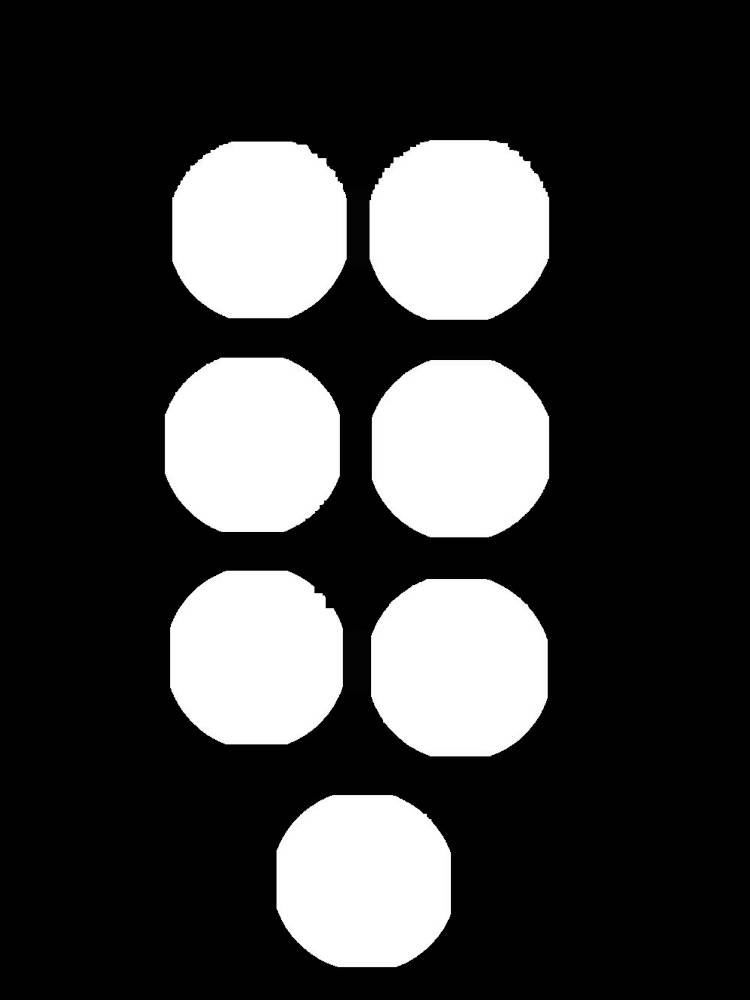
\includegraphics[width=7.5cm]{Imagenes/op_morf_monedas_final.jpeg} &
			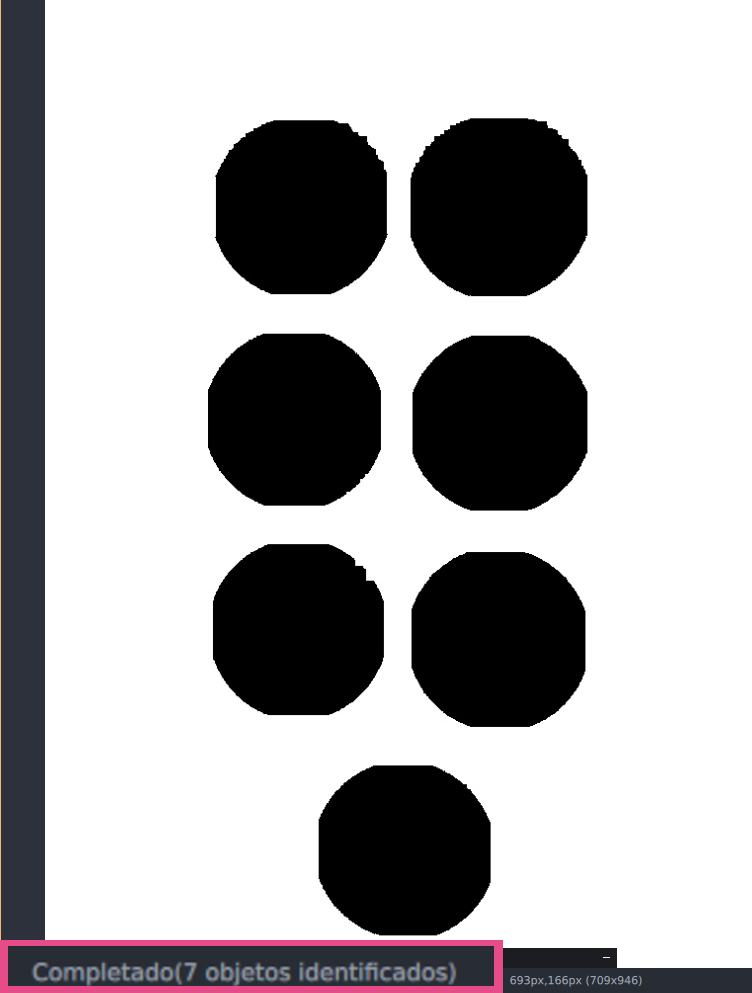
\includegraphics[width=7.5cm]{Imagenes/op_morf_monedas_contabilizacion.png}
		\end{tabular}
		\caption{1) Se encuentran casi en su totalidad separadas las monedas, resta eliminar esa unión utilizando la apertura con un kernel $n=9$. \\ 2) Se han rellenado y recuperado las monedas que había en un principio, sin embargo el tamaño aún no es el correcto por lo que deben aplicarse 7 dilataciones con kernel $n=12$.\\ 3) Una vez recuperada la forma y el tamaño casi original de las monedas se puede procesar y tratar la imagen como más se requiera, en este caso realizando la contabilización de los objetos. \\ 4) Importante señalar que típicamente los objetos se colorean de color negro y el fondo de color claro, por lo que la inversión de colores es requerida antes de invocar la contabilización.}
	\end{figure}
	
	\newpage
	
	\hfill\break
	\justifying
	La implementación de las operaciones morfológicas es bastante sencilla cuando se aprovechan las herramienta de la biblioteca OpenCV, existiendo ya como función las operaciones Erosión y Dilatación, a las cuales basta pasarles como argumento el elemento de estructura con su tamaño y forma especificada. Para la apertura y cerradura se cuenta con una función más general que recibe el tipo de operación a realizar identificado por una constante de la misma biblioteca y el elemento estructural como tercer argumento.

	\begin{lstlisting}[language=Python]
		def morphological_operation(morph_op_type:str,image,n:int=3,spatial_structure:str='rect',**kargs):
			image = copy(image)
			structuring_element = cv2.getStructuringElement(cv2.MORPH_CROSS if spatial_structure == 'cross' else cv2.MORPH_RECT,(n,n))
			
			if morph_op_type == 'erosion':
			return cv2.erode(image,structuring_element)
			elif morph_op_type == 'dilation':
			return cv2.dilate(image,structuring_element)
			elif morph_op_type == 'closing':
			return cv2.morphologyEx(image,cv2.MORPH_CLOSE,structuring_element)
			elif morph_op_type == 'opening':
			return cv2.morphologyEx(image,cv2.MORPH_OPEN,structuring_element)
	\end{lstlisting}

	
\newpage

\section*{6. Contrastado de Imagen}
	\hfill\break
\justifying
El dar contraste en una imagen implica cambiar el valor de cada uno de los pixeles en una imagen. Este cambio puede ser realizado por la multiplicación o división de los valores de los pixeles en la imagen utilizando una constane.

\hfill\break
\justifying
Utilizando la implementación ofrecida por OpenCV, para el aumento del contraste en una imagen basta asignar un valor positivo a la constante que se evalua en cada pixel. Con la misma lógica, un menor contraste implica un valor de constante positivo menor que 1.

\hfill\break
\justifying
El contraste y el brillo son elementos de las imágenes que pueden ser modificados y que tienen una relación cercana pero no se tratan de lo mismo, aunque suele ser complicado comprender cada uno sin una referencia que comparar.

\hfill\break
\justifying
Cuando en una imagen se ajusta el brillo, el rango entero de valores dentro de la imagen se alza o disminuye respectivamente. Una visualización sencilla de esto es tomando como referencia el histograma de una imagen en niveles de gris. Cuando se aumente al brillo, el histograma mantiene su distribución y forma, pero pareciera se recorre al lado izquierdo por que los valores anteriores de la imagen fueron modificados, aumentados, por la constante.

\hfill\break
\justifying
Cuando se cambia el contraste de una imagen, los tonos medios son eliminados. La imagen tendrá una porcentaje mayor de obscuros o negros, y blancos o resaltados con tonos medios mínimos. Recurriendo a la visualización con el histograma, cuando se contrasta positivamente una imagen, existe un aumento, la distribución de los valores se ensancha hacia los extremos, por lo que visualmente los elementos que se encuentren más separados en el nivel de grises, se verán más claramente cuando comparados. De la misma forma cuando el contraste es negativo, la distribución del histograma tiende a adelgazar y concentrar en un rango menor más valores pixeles.

\begin{lstlisting}[language=Python]
	def contrast(image,alpha:float=1.5,beta:float=0):
		return cv2.convertScaleAbs(image,alpha=alpha,beta=beta)
\end{lstlisting}

\hfill\break
\justifying
La aplicación del contraste con la biblioteca OpenCV se reduce a el manejo de los valores de las constantes $\alpha$ y $\beta$, donde $\alpha$ refiere al contraste y cada vez que se quiera operar directamente en el brillo sin cambiar este, su valor debe ser 1. La $\beta$ opera como la constante encargada de modificar el brillo de la imagen, valores elevados, relativamente, para este parámetro no son tan perjudiciales como puede ser un valor de contraste disparado. Si se desea modificar el contraste unicamente el valor de $\beta$ debe permanecer 0.

\newpage

\begin{landscape}
	\begin{figure}[!h]
		\centering
		\begin{tabular}{cc}
			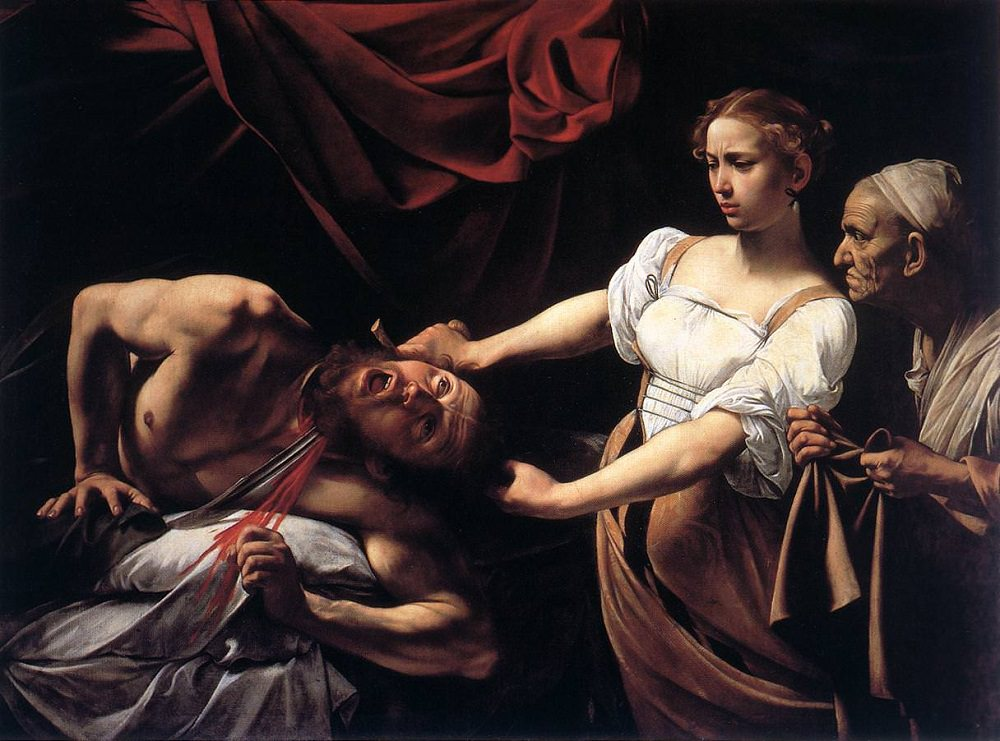
\includegraphics[width=12cm]{Imagenes/caravaggio.jpeg} & 
			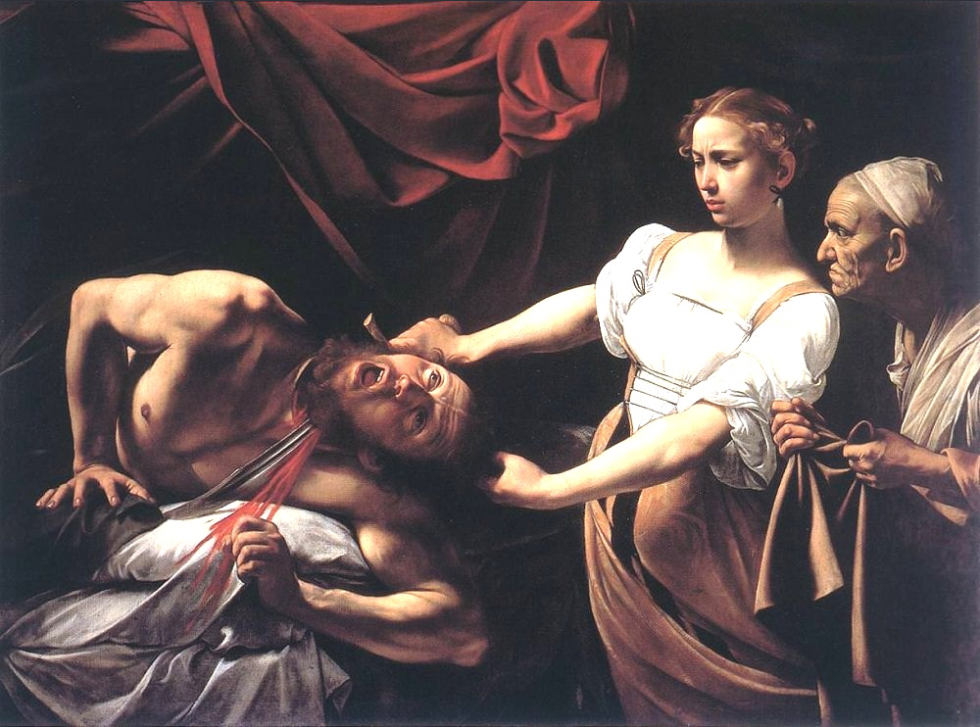
\includegraphics[width=12cm]{Imagenes/Contraste_ambos.png} \\
			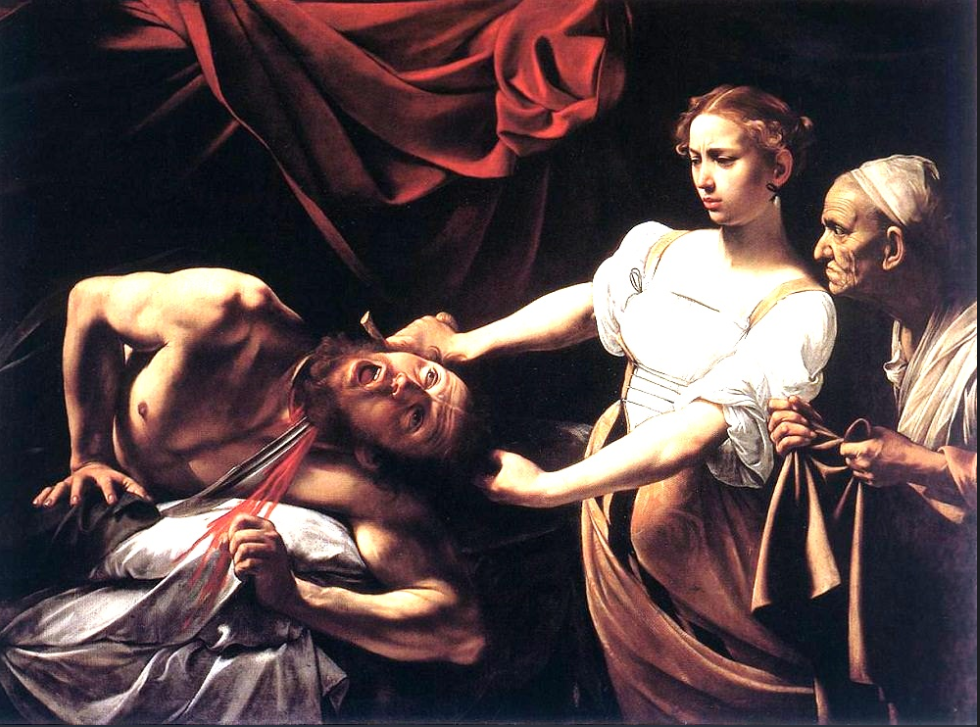
\includegraphics[width=12cm]{Imagenes/Contraste_contraste.png} & 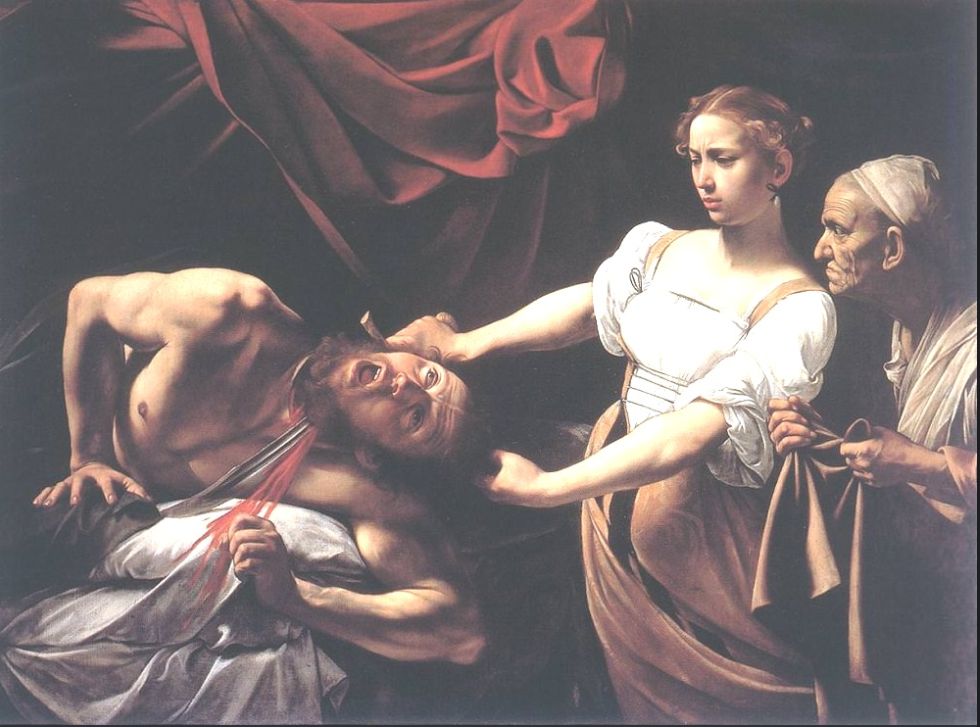
\includegraphics[width=12cm]{Imagenes/Contraste_brillo.png} 
		\end{tabular}
		\caption{1) Imagen original de la pintura 'Judit y Holofernes' de Caravaggio \\ 2) Imagen contrastada y aumentada en brillo respectivamente, con parámetros $\alpha = 1.2$ y $\beta = 30$ \\ 3) Imagen contrastada con $\alpha = 1.7$ \\ 4) Imagen con aumento de brillo $\beta = 70$}
	\end{figure}
\end{landscape}
	
\end{document}
